% $Id: thesis.tex 184 2013-10-23 14:59:01Z danbos $
% Author: Daniel Bosk <daniel.bosk@miun.se>
%
% These files may freely be used by students for their theses.
%
% If you make some improvements, please send a unified diff (`diff -u`) to 
% the author and it might be included in future revisions.
%
%\documentclass[a4paper,12pt,knd,final,oneside]{miunthes} % kandidat
%\documentclass[a4paper,bsc,final]{miunthes} % same as knd, B.Sc.
%\documentclass[a4paper,mag,final]{miunthes} % magister
%\documentclass[a4paper,msc,final]{miunthes} % same as magister, M.Sc.
\documentclass[a4paper,12pt,mst,final, oneside]{miunthes} % bologna master, M.Sc.
% \documentclass[a4paper,project,final]{miunthes} % generic project report


%%%%%%%%%%%%%%%%%%%%%%  BASIC packages  %%%%%%%%%%%%%%%%%%%%%%%%%%%%%%%%%%%%%%%%
\usepackage[top=1in, bottom=1.25in, left=1.25in, right=1.25in]{geometry} % center onesided report

\usepackage[T1]{fontenc}
\usepackage[utf8]{inputenc}
\usepackage[swedish,english]{babel}

\usepackage[intoc]{nomencl}
\usepackage{varioref,prettyref}
\usepackage{url}
\usepackage{amsmath,amssymb,amsthm}
\usepackage{listings}
\usepackage{nameref}
\usepackage{longtable}
\usepackage{float}
\usepackage{listings}
\usepackage{enumitem}                       % spacings in the list
\usepackage{setspace}						% change line spacing
\usepackage{ifthen}                         % ifthenelse cmd
\usepackage{pgfkeys}                        % command key => value approach, ex: \cmd[width=10cm]{hej}
\usepackage[printonlyused]{acronym} 		% Acronyms
\usepackage[hidelinks]{hyperref}			% turn acronyms, ToC, figure and table captions into hyperlinks, but hide the links, but don't highlight the links
\usepackage[capitalise,noabbrev]{cleveref}	% This one is awesome! Automatically recognises the object referred to (use for Lables, Images, Tables, etc.)

\usepackage{pdfpages}                       % To include the front page
%% tikZ Graphic Package
\usepackage{standalone}			% include standalone files (tikZ pictures from external files, etc)
\usepackage{tikz}
\usepackage{xcolor}
\usetikzlibrary{shapes.geometric,arrows.meta}
\usepackage[utf8]{inputenc}
\usepackage{pgf, tikz}			% tikZ drawing package
\usepackage{pgf-umlsd}
\usetikzlibrary{calc,arrows,automata,shapes}	% tikZ libraries
\usepackage{algorithm}
\usepackage[noend]{algpseudocode}
\usepackage{multirow}
\usepackage[style=numeric-comp,natbib=true,maxbibnames=99,sorting=none,backend=biber]{biblatex}

%%%%%%%%%%%%%%%%%%%%%%%%%%%%%%%%%%%%%%%%%%%%%%%%%%%%%%%%%%%%%%%%%%%%%%%%%%%%%%%%%%%%%%

%\setcounter{secnumdepth}{4}    in miunthes.cls
%\setcounter{tocdepth}{4}


\renewcommand{\comment}[1]{}
\newcommand{\newpara}{\\[0.3cm]}
\newcommand{\course}{dist}

\addbibresource{library.bib}
\usepackage[varioref,prettyref,listings,nomencl]{miunmisc}
\makenomenclature
%
\subject{Computer Engineering}
\title{Master's thesis}

\subtitle{
    Department of Information Systems and Technology
    \newline
    \newline
    Master of Science in Computer Engineering
    \newline
    %\textsl{\normalsize{Master by Research in Computer Engineering}}
    \newline
    \newline
    \newline
    \textbf{Context-Based Authentication and Lightweight Group-Key Establishment Protocol for IoT Devices}
    \newline
}

\author{Nico Ferrari}
%\setboolean{@twoside}{false}


\begin{document}

%\includepdfmerge{out/Bsc_thesis_front_page.pdf,-}
 	\begin{titlingpage}
 		\maketitle
 	\end{titlingpage}
	\frontmatter
	\noindent
	\vspace{\fill}\\
	\textbf{MID SWEDEN UNIVERSITY}\\
    Department of Information Systems and Technology\\
    \newline
    \textbf{Examiner:} Prof. Mikael Gidlund, \url{mikael.gidlund@miun.se}\\
    \textbf{Supervisor:} Dr. Ulf Jennehag , \url{ulf.jennehag@miun.se}\\
    \textbf{Author:} Nico Ferrari, \url{nife1600@student.miun.se}\\
    \newline
    \textbf{Degree program:} Master of Science in Computer Engineering, 
        \newline   Master by Research, 120 ECTS \\ 
    \textbf{Main field of study:} Computer Engineering\\
    \textbf{Semester, year:} Summer, 2019 \\
    \textbf{Release date of this thesis report:} \today
    
    
    \clearpage
    
    %\input{text/docversions.tex}
    %\clearpage
    
	%\include{abstract-sv}
	%\cleardoublepage
	% $Id: abstract-en.tex 142 2012-12-22 10:41:32Z danbos $
\begin{abstract}
	\noindent
The concept of the Internet of Things is driven by advancements of the Internet with the interconnection of heterogeneous smart objects using different networking and communication technologies. 
With the rapidly increasing number of interconnected devices present in the life of a person, providing authentication and secure communication between them is considered a key challenge.
The integration of Wireless Sensor Networks in the Internet of Things creates new obstacles due to the necessity of finding a balance between the resources utilization and the applied security solutions.
In multicast group communications, the energy consumption, bandwidth and processing overhead at the nodes are minimized in comparison to a point-to-point communication system.
To securely transmit a message in order to maintain confidentiality of the data and the user's privacy, usually involves human interaction or the pre-agreement upon some key, the latter unknown to an external attacker. 
In this thesis, the author proposed an authentication protocol based on the similar context between the correct devices and lightweight computationally secure group-key establishment, avoiding any kind of human involvement.
The goal is achieved by having the devices calculate a fingerprint from their ambient context and through a fuzzy commitment scheme generating a commitment respectively opening value which is used to generate a common secret key between them.
The tests are effectuated on real world data accumulated from different environments.
The proposed scheme is based on elliptic curve cryptography and cryptographic one-way accumulators. 
Its feasibility is analyzed by implementing the group key establishment phase in the Contiki operating system and by simulating it with the Cooja simulator. 
Furthermore, the applicability of the protocol is analyzed and justified by an analysis of the storage overhead, communication overhead, and energy consumption.
The simulator shows an energy consumption of only  112 mJ per node for group key establishment.
The results obtained in this thesis demonstrate the feasibility of the scheme and its computational and communication costs are further comparable to other similar approaches.


	\keywords{Internet of Things, Context-based authentication, Fuzzy commitment scheme, Cryptographic  key  establishment,  Lightweight  cryptography,  Contiki,  One-way  accumulators}
\end{abstract}








	\clearpage
	
	\chapter{Acknowledgement}
\label{ch:acknowledgement}
Foremost, I would like to express my sincere gratitude to my supervisor Ulf Jennehag for the continuous support during my Master studies. 
Thanks to his patience, motivation and enthusiasm which guided me during my studies and supported the participation the two conferences in Valencia and in Sundsvall.
\\
\\
I would also like to express gratitude to Teklay Gebremichael for reviewing the thesis. Thank you for being always ready to advice me, to help me to clear doubts and for all your great feed-backs during these years.
\\
\\
Heartfelt thanks go to Thomas Wiss which gave me invaluable help with proof reading the thesis report. Thank you for listening, offering me advice, and supporting me through this entire process. 
From the deep of my  heart I thank you for your friendship.
\\
\\
Next, I would like to thank the friends and nice people from all over the world that I met during these amazing years and for all the memories we shared.
\\
\\
Finally, my deep and sincere gratitude to my family for their continuous support, help and love.
I am forever indebted to my parents for giving me the opportunities, encouraging me to engage new challenges and inspiring me to follow my dreams.
This would not have been possible without them.
Thank you.
% Don't thank the examiner!




	\clearpage
	%\cleardoublepage
	%\include{preface}
	%\cleardoublepage
	\tableofcontents
	\clearpage
	
	\iffalse
\chapter{List of Publications}

This master's thesis has in addition the following two publications of the author in full-text form at the end of the report included:

\begin{enumerate}[label=\Roman*]
    \item T.Wiss, S. Forsstr{\"o}m. "Performance Evaluation of Secure CoAP and MQTT Communication on Resource-Constrained Devices". In \textit{The 13th Swedish National Computer Networking Workshop in Halmstad, 2017}, pp. 42-45.
\end{enumerate}


\fi


	
	\chapter{Terminology}

\iffalse
\section{Terms}

\begin{table}[h!]
\centering
\small
\def\arraystretch{1.6}
 \begin{tabular}{ m{4.5cm}|m{10cm} }
     \hline
     \textbf{Term} & \textbf{Explanation}  \\ 
     \hline
     Node & A node is a redistribution or communication endpoint. In distributed systems nodes can be clients, servers, or peers.  \\ 
     Communication model &  A conceptual model applied to interpret communication processes where communication is the process of transferring information from one part (sender) to another (receiver). \\ 
     Topic & A topic is a term used in the publish/subscribe communication model and describes a computational resource containing and storing information.   \\ 
     End-to-end test & A software testing method to determine if a flow of an application is executing as determined from start to finish. \\ 
     Unit test &  A software testing method to determine if an individual unit or block is operational. \\ 
     Response time & The response time is the time passed between an inquiry on a system and the response to that inquiry. \\
     Bandwidth consumption &  The amount of bandwidth required and applied to transmit a message. \\ 
     Communication overhead &  The amount of additional resources required to transmit the actual message content.  \\ 
     \hline
 \end{tabular}
\end{table}



%\section{Mathematical notations}
% Only if needed 
\clearpage
\fi
\section{Abbreviations and Acronyms}
\addcontentsline{toc}{section}{Acronyms}
\begin{acronym}[TDMA]
	% use \acs for singular and \acsp for adding an s (plural)
	% use \acfi to write the full name and the acronym in ()
	\acro{5G}{Fifth Generation}
	\acro{AES}{Advanced Encryption Standard}
	\acro{CRNG}{Common Random Number Generators}
	\acro{DH}{Diffie-Hellman}
	\acro{ECC}{Elliptic Curve Cryptography}
	\acro{ECDH}{Elliptic-Curve Diffie-Hellman}
	\acro{ECDLP}{Elliptic Curve Discrete Logarithm Problem}
	\acro{EC}{Elliptic Curve}
	\acro{HMAC}{Hash Message Authentication Code}
	\acro{IEEE}{Institute of Electrical and Electronics Engineering}
	\acro{IIoT}{Industrial IoT}
	\acro{IoT}{Internet of Things}
	\acro{OTP}{One-Time Pad}
	\acro{PKC}{Public Key Cryptography}
	\acro{RPi}{Raspberry} {Pi}
	\acro{RS}{Reed-Solomon}
	\acro{WSN}{Wireless Sensor Network}
	\acro{ZIA}{Zero Interaction Authentication}
\end{acronym}



\clearpage


	
	%\cleardoublepage
	%\listoffigures
	% \cleardoublepage
	% \listoftables
	%\cleardoublepage
	%\lstlistoflistings
	%\printnomenclature
	
	\mainmatter
	
	% $Id: introduction.tex 142 2012-12-22 10:41:32Z danbos $
\chapter{Introduction}
\label{ch:introduction}

During the last decades Internet has evolved significantly towards the Internet of Things (\acs{IoT}) environment, where  different resource-constrained objects  communicate and exchange information with each other for improved functionalities and performance. 
The Internet of Things denotes the interconnection of highly  heterogeneous  networked  embedded systems  (nodes)  with different communication patterns, enabling the connection to IP networks and allowing them to be remotely monitored and controlled \cite{Heer2011}.
According to the projections made by networking specialists, it is forecast that by the next years the adoption of \acs{IoT} will boost the amount of connected devices, estimating many billions of different web-enabled devices all around the globe\cite{Chen2014} \cite{CiscoInternetBusinessSolutionsGroupIBSG2011TheEverything}.
IoT introduces different changes to the future of Internet, becoming also a key enabling technology of the Fifth Generation(\acs{5G}) wireless systems.
This development does not only affect digitalizing and connecting the society, but also the industry and economy as a whole. 
Concepts brought by the Internet of Things, such as IoT cloud computing, Big Data analysis on data gathered from the sensors, reached also the industry which has started to embrace the IoT forming the Industrial Internet of Things (\acs{IIoT}) \cite{Shrouf2014SmartParadigm}.

With the development and expansion of communication and sensing technologies, also the research sector has been affected, bringing new challenges.
The main research challenges moved, in fact, from packet switching to connect several computers in a network \cite{Barry2015BriefInternet}, trying to make devices accessible and allowing communication between them.

Over the last two decades, wireless communications and digital electronics technologies have been rapidly evolving by introducing the incredible advances to Wireless Sensor Networks (\acsp{WSN}).
Typically, a \acs{WSN} is a network that comprises a large number of sensor nodes, where each node is equipped with single or multiple sensors to detect physical phenomena such as light intensity, temperature, humidity, or pressure measuring and quantifying their physical environment \cite{Akyildiz2002WirelessSurvey}.
\acsp{WSN} represent an important technology for distributed monitoring of different physical quantities, capable to provide measurements characterized by high temporal and spatial resolutions.



\section{Background and problem motivation}
\label{sec:background}
The more objects are connected the more the network is exposed to security vulnerabilities, leading to a drastic exposure of users' potentially sensitive privacy threats.
Considering, therefore, the number of everyday device which could possibly be involved, the \acs{IoT} has greater threats and risks than what Internet has until now\cite{NationalIntelligenceCouncil1385Six2025}. 
Security and privacy attacks and their harmful consequences can occur when sensitive information is concealed or controlled without users' consent.

Despite the fact that security is a prime and mandatory requirement that should be integrated at the design phase of the \acs{IoT} device life-cycle, still it is too often neglected in the development of systems. 
Recent press reports highlight many security breaches that are taking the advantage of insecure \acs{IoT} devices, leading attacks such as against networked garage or cars  door systems \cite{Eisenbarth2008OnScheme} or medical devices \cite{Strobel2013FumingSystem}.

Due to the heterogeneously of the networking technologies and devices in dynamic networking environments, the deployment of conventional security protocols has become challenging.
In fact, to face powerful attackers, devices with high performances require advanced security solutions.
However, these protocols can be too expensive to be deployed on resource constrained devices, which are limited in terms of battery capacity, computational power, memory-footprint and bandwidth utilization.

Moreover, even traditional cryptographic techniques, such as the \ac{DH} protocol, are not sufficient for a secure pairing between the devices that spontaneously come into the network.
Techniques like the devices' names and network addresses do not guarantee protection from the devices impersonation by an attacker.

Therefore, finding a balance between security solutions and the associated resources utilization overhead is subject to new challenges, keeping regard on how these systems can be made easily usable and not compromised by users.

Since there is a enormous amount of connected devices with different functionalities, it may happen that some have to communicate with an unknown number of other devices.
Clustering and multicasting result the most efficient means of resource management in the communication in IoT applications \cite{Klaoudatou2011AWSNs}.
In group communication a group of two or more devices communicate with each other in such a way that a sender broadcasts a message to the group rather than sending a unicast message for each group member.
Conveying messages to a multicast group is more efficient and effective than sending unicast messages to different devices in multiple copies. 
Multicast communication helps with improving the bandwidth usage reducing the number of transmitted messages and enabling then a fast delivery of a message to multiple recipients, a very important feature in time critical applications.
It also minimizes the energy consumption and processing overhead at the terminals improving their lifetime and responsiveness. 


\section{Problem statement}
\label{sec:problemstatement}

According to the statistics \cite{statIoT} there are more than 7 billions of connected "things" in the world today, challenging the researchers with novel research problems due to this ever-growing amount of devices. 
%%statistics (https://iot-analytics.com/state-of-the-iot-update-q1-q2-2018-number-of-iot-devices-now-7b/)%%
%It becomes important to establish  security  associations  with  devices  that  are introduced into the user’s trust domain and efficiently identify them. 

The thesis aims to address the following research questions:
\begin{itemize}
    \item[RQ1:] How can lightweight and secure key establishment and authentication protocols be designed in order to permit the deployment on constrained devices in IoT applications?\\Public  key  cryptography (\acs{PKC}) has usually been chosen to ensure a satisfactory level of  security  for  data  transmissions  within  the  network.  
    This is  because  one  does  not  need  to  transmit  the  private  key in  the  channel,  in  addition  to  providing  digital  signatures that can not be repudiated. 
    However, the constrained energy, computation,  and  memory  budgets  of  sensors  make  the implementation of PKC challenging.
    
    \item[RQ2:] Can the physical environment be exploited in order to enable secure authentication between devices and gateways?\\
    During the last years, the constantly increasing number of sensors in combination with the variation inherent in many of the measurable quantities, brought into the spotlight novel security approaches(such as Common Random Number Generators \acs{CRNG}). 
    Using the aquired data to generate mutual authentication could bring a natural way to authenticate that the keys obtained through the cryptographic exchange belong to devices that are within phisical proximity.
    The pairing would happen without user interaction, based solely on information that the involved devices can communicate and sense from their ambient context without human involvement.  
    
\end{itemize}
The research questions of this study which are outlined above are motivated by the research problems described in the previous sections.

\section{Scope}
\label{sec:scope}
The scope of this thesis work is to analyze the use of context information in order to  realise autonomous establishment of security services able to be used by the IoT applications mentioned previously.
The target of the authentication protocol are IoT devices in factory and office environments and the complexity of the services is not the scope of this research.
For the group-key establishment protocol the target are wireless sensors in order to being able to extend the solution to more powerful devices. 
The evaluations are performed on simulated devices and the implementation of the proposed solutions on physical devices is not included as part of this work.

The conducted implementations of the concepts proposed in the thesis are considered a Proof of Concept, therefore is not included efforts to provide production ready solutions. 
The power efficiency related properties (e.g. duty-cycle) are also out of the scope of this thesis. 
Power consumption result is only measured for key establishment process. 
In order to reduce the measurement loads, each devices are configured to disable the power saving option. 
Each devices has 100\% active time and resulting always on ready state to receive, send and process a message.

\section{Concrete and verifiable goals}
\label{sec:goals}
As part of the preparation and initialization of the master thesis project work a set of concrete and verifiable goals has been elaborated and is presented in the following list:
\begin{itemize}
    \item[G1] Research and evaluate context-based authentication and lightweight group key management protocols used in the IoT context. 
    \item[G2] Implementation of devices able to get ambient data using different sensors and data acquisition from real world use cases.
    \item[G3] Analysis of the obtained data in order to generate an authentication key between devices in located in the same ambient.
    \item[G4] Design and implementation of a lightweight group-key management scheme which uses lightweight cryptographic primitives.  
    \item[G5] Measure the computation overhead and the communication overhead of the implemented protocol and include related lightweight group-key management protocols in the performance evaluation.
\end{itemize}
How these goals were achieved as part of the work in this master thesis project is outlined in the subsequent chapters. First however, an outline of the chapters in the report at hand is provided.


\vspace{2em}

\section{Outline}
\label{ch:disposition}
Chapter \ref{ch:introduction} introduces the topic of this master thesis project, gives reasons for the project's motivation, scopes the work, and sets goals to be achieved in this master thesis project. The following Chapter \ref{ch:theory} outlines and describes the principle topics encountered during the master thesis project. Chapter \ref{ch:methodology}, Methodology, describes in which manner the concrete goals shall be approached in order to fulfill them. The Chapter \ref{proxAuth} describes the scenarios analyzed for the context-based authentication scheme and the threat model considered in the study. The subsequent Chapter \ref{ch:implementationAuth} gives detailed insight into the implementation efforts conducted in this master thesis project work related to the authentication protocol. Chapter \ref{ch:lightwightProto} is described the proposed lightweight group-key establishment protocol and the implementation details are shown in Chapter \ref{ch:implementationProto}. The results of the performance evaluation of the authentication protocol and the proposed group-key management scheme are covered in Chapter \ref{ch:results}. The final chapter, Chapter \ref{ch:conclusion}, outlines the thesis' conclusion which contains a discussion covering the implementation efforts and tests, the conclusion itself and further describes both the ethical considerations and the potential future work. 




%%%%%%%%%%%%%%%%%%%%%%%%%%%%%%%%%%%%%%%%%%%%%%%%%%%%%%%%%%%%%%%%%%%%%%%%%%%%%%%%%%%%%%%%%%%%%%%%
%   The old stuff but maybe still important
%%%%%%%%%%%%%%%%%%%%%%%%%%%%%%%%%%%%%
\iffalse


\section{Background and problem motivation}
\label{sec:background}
%Investigate and examine the performance of IoT application layer protocols in general and combinations of various protocol stacks.
%Why? Able to compare existing IoT protocols, make adaptions and choose appropriate protocol for given situations.

--REWRITE
The Internet of Things (IoT) is an emerging technology movement towards connecting devices in the scale of billions in the near future\cite{Evans2011}. The IoT is one of the fundamental parts for the construction of the "Industry 4.0" \cite{Shrouf2014}. In addition, it has the possibility to influence the activities of a people in almost any aspect of their lifes\cite{Atzori2010}. 

However, many topics in the IoT such as the network architecture, addressing, or security are still open issues\cite{Borgia2014}. Yet different architectures have been proposed to cope with the complex, versatile IoT scenarios. One of those approaches has the principal idea of combining the enormous computational resources of the cloud with the things in the IoT. This introduces many advantages such as on-demand and scalable storage yet introduces many new challenges and issues to overcome. One of the foremost mentioned issues is the unsatisfied high latency \cite{Yi2015} which is introduced by the long physical distances between the sensing devices and the cloud. Another challenge is the enormous amount of sensed data which needs to be transmitted through the Internet backbone. These limitations of the architectural solution are currently subject of research.





\section{Overall aim}
\label{sec:overallaim}
%improve the qos. more variations to pick from for different IoT situations.

-REWRITE, does this belong here?
Not only can this research enable the utilization of SCTP for future applications in the fog computing environment to enhance the reliability and failure-resilience, moreover, it may present a practicable alternative to the well-established transport layer protocols TCP and UDP. 
The outcome of this research study has furthermore the potential to serve as a basis for enhanced experiments and feasibility tests of the SCTP protocol such as the influence of a secure data transmission. It offers the chance to conduct trials and research of the utilization of SCTP for IoT application layer protocols such as CoAP or the Message Queuing Telemetry Transport protocol (MQTT) \cite{specMQTT}. Furthermore, the opportunity is presented to design and build an exclusive, first of a kind application/library, which applies the SCTP protocol on the transport layer, to transmit and exchange sensed data in a IoT/fog computing environment.

Yet this study could also identify as well as giving reasons why or to which degree the SCTP protocol is not applicable in the fog computing environment or in specific situations. 

Whichever outcome the study shows, the research community can benefit of the results and apply the findings towards providing a higher QoS respectively QoE in a fog computing environment for the user, industry, or business sector.


!!!!
USE THE STUFF FROM THE PROPOSAL!!!!!!!!!!
!!!!!!
-->> and have a look at the other thesis project reports



\section{Scope}
\label{sec:delimit}
%limited to IoT on medium constrained devices such as Raspberry Pi
%protocols and network performance metrics

%Focus on the protocols for the communication between parties involved in the IoT, sensor devices, middle layer devices and the cloud is the decided upon general direction of research.


\section{Concrete and verifiable goals}
\label{sec:goals}
--REWRITE, does this belong here??
The first aim is to examine the feasibility of the SCTP protocol for a utilization in a fog computing environment. This can be achieved by conducting an extensive research of existing work and conduct a theoretical/elementary suitability test. Secondly a comparison of TCP, UDP, and SCTP in a qualitative as well as quantitative manner can be conducted to evaluate the performance of the protocols regarding a utilization in a fog computing environment. As a next step, an implementation of a fog computing testbed can be pursued to compare the performance of the above-mentioned protocols and in combination with an IoT application layer protocol such as CoAP or other kinds of applications. Further tests and experiments evaluating the QoS of all the applied implementations will be included in this step.
To this end, the comparison can be extended to include the provided secure data transmission systems of the evaluated protocols and implementations.



\section{High-level problem statement}
\label{sec:aim}
%The application areas of the IoT are as manifold as it gets. No solution will fit it all. It will rather be an assortment of many different technologies, protocols and devices. 
%\cite{atzori2010internet} depicted 5? main areas were the IoT will be applied

%Therefore one needs to investigate and examine various ways of fulfilling a given task respectively situation. 

--REWRITE
The purpose of this study is to find means and potentials to enhance the QoS of the fog computing architecture to make it more applicable for industry or business solutions. 

Being able to serve a situation- and business-aware QoS for a given field or area is one of the challenges which need to be solved to allow the fog computing approach a widespread utilization. Furthermore, it is important to note that the QoS is not only a technical/engineering issue since it involves the needs and requirements of the users and customers. An offered implementation is therefore closely coupled to the business side and has an influence on the profit of the offered application. 
Since the mere nature of the IoT is to be applicable in almost any domain, the QoS-metrics may vary heavily depending on the applied field and situation. It is therefore a reasonable approach to investigate the influence of certain QoS-metrics in different situations and find means to improve the QoS in these situations. Hence the examinations, experiments, and enhancements are in most cases tightly coupled to the applied scenario. 

Not always directly part of the QoS is the security and protection of the sensed data yet should this topic have at least a basic coverage in every applied work in this study. This is, since the acceptance of the IoT and therefore fog computing is, to a certain portion, based on the ability to provide the user, industry, and business a secure solution to their problem. 


\section{Detailed problem statement}
\label{sec:problemstatement}



\section{Outline}
\label{ch:disposition}
Chapter 2 describes ..
Chapter 3 describes ..

\fi
%%%%%%%%%%%%%%%%%%%%%%%%%%%%%%%%%%%%%%%%%%%%%%%%%%%%%%%%%%%%%%%%%%%%%%%%%%%%%%%%%%%%%%%%%%%%%%%%%%%%%%%%%%%%%%%%%%%%%%%%






%%%%%%%%%%%%%%%%%%%%%%%%%%%%%%%%%%%%%%%%%%%%%%%%%%%%%%%%%%%%%%%%%%%%%%%%%%%%%%%%%%%%%%%%%%%%%%%%%%%%%%%%%%%%%%%%%%%%%%%%
\iffalse
%%%%%%
\section{Contributions}
\label{ch:contrib}

--- There were no other contributer in this project. So don't include this section, not even the title.



\noindent
This project had two contributing workers, Johannes and Thomas. The division of the work was to let Thomas work on the private cloud setup with the open source system OpenNebula and integrate the gaming service on a public cloud (Amazon AWS). Thomas also had the responsibility to add HTML and CSS code for the visual experience in the service as well. He made it responsive for small screen mobile devices as well as for large screens on desktops. 
\newpara
Johannes on the other hand setup the service itself and programmed most of the back-end and front-end of the game service as well as the listing. He constructed a basic game simulation on the server side for the game environment and it's properties to render to a canvas image instead of the screen. He constructed a stream of the generated game images to send to the client and an API for controlling the game from the client side.
\newpara
There was a lot of corporation between the two participants in the project, the evaluation and the measurements of the streaming, which was done completely together.

\fi
	% $Id: theory.tex 142 2012-12-22 10:41:32Z danbos $
\chapter{Theory}
\label{ch:theory}
In this chapter technologies and topics of relevance for this thesis project work are outlined and explained. It offers a gradual introduction into the technologies and topics applied.

\section{Fuzzy Commitment Scheme}
Traditional cryptographic systems rely on keys, secret sets of bits used for secure management of data. 
For example, a symmetric-key cipher involves a secret key \textit{x} and two operations defined as encryption and decryption.
The encryption function takes as input a message \textit{m} and the key \textit{x} and returns as output a cyphertext \textit{c}.
The decryption function reverses the encryption, taking as input the cyphertext \textit{c} as well as the key and yielding the original message \textit{m}.

Ordinary ciphers rely on exact correctness of the key \textit{x}, making possible the decryption of a cybertext \textit{c} only with a precise key.
Fuzzy commitment, however, is a cryptographic primitive which as has been designed by Juels and Wattenberg \cite{Juels2004AScheme} in order to handle noise over the key \textit{x}.
A commitment scheme is defined as a function $G : C \times X \xrightarrow{} Y$ able to commit a random secret value $\kappa \in C $ choosing a witness $x \in X$ and computing a \textit{blob} value  $y = G(\kappa,x)$.
A decommitment function $G^{-1}: Y \times X \xrightarrow{} C$ takes a blob and a witness as input and yields the original value $\kappa$.
A well defined commitment scheme shall have two basic properties:
\begin{itemize}
    \item binding: it is not possible to decommit $y$ under a pair $(\kappa', x')$ such that $\kappa' \neq \kappa$ ;
    \item hiding: given $y$ alone, it is infeasible to compute $\kappa$.
\end{itemize}
The fuzzy commitment encryption scheme allows the recovery of $\kappa$ from a given commitment $y=G(\kappa, x)$ from any witness $x'$ close to $x$ in some appropriate metric, such as Hamming distance, but not necessarily identical to $x$.
Since $h(c)$ is a secure one-way function, $y$ leaks only a small amount of information about a committed value, therefore it may be revealed publicly and used to recover $\kappa$ using any close witness $x'$.

The $n$-bit witness can be expressed  in terms of the committed value with an $n$-bit offset $\delta$ such that $x = \kappa \oplus \delta$. The idea behind the commitment function $G$ is to hide $\kappa$ using an hash function $h$ (such as SHA256) while leaving $\delta$ in clear. 
The commitment function can be then defined as:
\begin{center}
    $G(\kappa,x) = (h(\kappa), x \oplus \kappa) = (h(\kappa), \delta)$
\end{center}
It is then possible to leverage the error correcting properties of error correcting codes such as \ac{RS} to correctly recover the secret $\kappa$.
An error-correcting code comprises a message space $C \subseteq \{0,1\}^a$ , a corresponding codeword space $C \subseteq \{0,1\}^b$ , for $b \geq a$, and a bijection $\varphi : M \longleftrightarrow C$. 
Here $\{ 0, 1 \}^k$ denotes a $k$-bit message/codeword generating a space with a total of $2^k$ distinct elements.
Another important element of error-correcting codes is a decoding function $f:C' \xrightarrow{} C \cup \bot$, where $C \subseteq C' \subseteq \{0,1\}^b $.
The role of the decoding function is to map an element in $C'$ to its nearest (i.e., nearest in terms of Hamming distance) element in $C$, resulting in the elimination of the noise added to a codeword or the failure to find a valid one, denoted with the symbol $\bot$.


To decommit $F(\kappa,\delta)$ using a witness $x'$ , the receiver computes $\kappa ' = f(x' \oplus \delta)$ , where $f$ is an efficient decoding function from the error correcting code.
If the received $h(\kappa)$ corresponds to $h(\kappa ')$ then the blob has been successfully decommitted, with $\kappa '$ representing the extracted commitment, otherwise, $x'$ represents an incorrect witness. 

One application of fuzzy commitment, as suggested by the authors in \cite{Juels2004AScheme}, is to secure biometric systems.
An enrolled fingerprint image (known as a template), for example, might be viewed as a key $x$. The user tries to authenticate using another, slightly different image of the same finger,which we may denote by $x'$. Authentication is successful if and only if $x'$ is "close" to $x$.

%%%Fuzzy extractors are used to convert biometric data into random strings which can be applied in cryptographic techniques for biometric security. 
%One of the first fuzzy extractors systems is \textit{Fuzzy commitment} \cite{Juels2004AScheme}, designed by Juels and Wattenberg, where, using biometric data "close" to each others, is possible to decommit a cryptographic key.
%The idea is to bind a string of random bits with a biometric template in binary format called difference vector.
%Ideally, it is infeasible to recover the difference vector either the biometric template or the random bit string without any knowledge of the user's biometric data.

\section{Elliptic Curves Cryptography}
\label{theory:ECC}
Elliptic curve cryptography is a public key cryptosystem developed by Neil Kobiltz and Victor Miller in 19th century \cite{Miller2000TheCryptography}.
An elliptic curve (\acs{EC}) over the field $\mathbb{F}$ is the set of all solutions (x,y) in $\mathbb{F}$ that satisfy the mathematical equation:
\begin{equation}
y^2 + a_1xy + a_3 y = x^3 + a_2 x^2 + a_4 x + a_6
\end{equation}
where $a_1,a_2,a_3,a_4,a_5,a_6 \in \mathbb{F}$ together with a point at \textit{infinity} denoted by $\infty$.
Cryptographic systems usually use elliptic curves over prime fields $\mathbb{F}_p$ ( for some large prime number $p$) or binary fields ($\mathbb{F}^m_2$ for some integer $m$ ), since field arithmetic in these particular fields can be implemented very efficiently. 
For the purpose of this thesis, we have focused on prime field curves recommended by the National Institute of Standards and Technology (NIST) using implementation following these standard practices. 
In curves over a prime field, the \textit{Weierstrass} equation above can be expressed, using a variable change, as a much simpler equation of the form

\begin{equation}
y^2 = x^3 + ax + b
\label{ec_formula}
\end{equation}

The set of points $x,y \in \mathbb{F}$ that satisfy equation \ref{ec_formula}, plus the point $\infty$ and an "addition" form a group \cite{Washington2008EllipticApplications}.
To perform the operation of addition of two points $\mathbb{P}(x_1,y_1) \neq \mathbb{Q}(x_2,y_2) $ and  $ \mathbb{P},\mathbb{Q}\neq \infty$ on the curve $E(a, b)$ to obtain a third point $R(x_3, y_3)$ on the curve, we need draw a straight line that passes through the two points. 
The line will intersect the curve in another point $-\mathbb{R}$. 
Reflecting across the x-axis that point, we find the third point, $\mathbb{R}$, as shown in Figure \ref{fig_ec}. 

\begin{figure}[!h]
\centering
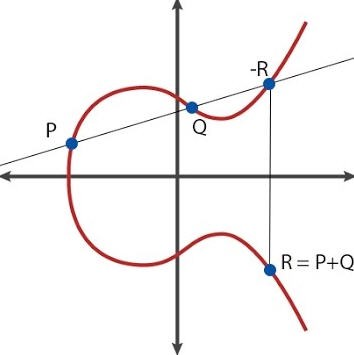
\includegraphics[width=3in]{images/ecc.png}
\caption{Group law on an elliptic curve.}
\label{fig_ec}
\end{figure}

In the case where $\mathbb{P} = \mathbb{Q}$, we will draw a line tangent to that point and then looking for the point which intersects with the curve. Its reflection along the x-axis is the sum $\mathbb{P} + \mathbb{P}$.
If $\mathbb{P} = \mathbb{Q}$ with $y=0$ or $y_1 \neq y_2$, the sum will be $\mathbb{P} + \mathbb{Q} = \infty$.
A related group operation is the scalar point multiplication, where by a given point is added to itself a given number of times.

The security of elliptic curve cryptography rests on the assumption that the \ac{ECDLP} is hard, which represent the fundamental building block for \acs{ECC}.
The ECDLP is the following computational problem:
given points $\mathbb{P}, \mathbb{Q} \in \mathbb{E}$ to find an integer $a$, if it exists, such that $\mathbb{Q} = a \mathbb{P}$.

Elliptic Curve Cryptography (ECC) is a preferred choice among various PKC options due to its fast computation, small key size, and compact signatures\cite{Research2000}. 
Experiments proved that Elliptic Curve Cryptography (ECC) is more suitable for resource constraint devices compared with RSA \cite{Gura2004}\cite{2005EnergyNetworks}.
For example, to provide equivalent security to 1024-bit RSA, an ECC scheme only needs 160 bits on various parameters, such as 160-bit finite field field operations and 160-bit key size\cite{Research2000}. 
EC parameters are denoted by \textit{a, b, q, p and $\mathbb{P}$} and they are embedded in all the entities that participate in the communication scenario. 
The parameter q is the prime which indicates the finite field $\mathbb{F}_q$. 
The variables $a$ and $b$ are the coefficients of the elliptic curve. 
$\mathbb{P}$ is the base point generator with order $p$ which is a  prime number.

\section{One Way Accumulators}
%We build a secure group membership operation by using one-way accumulators \cite{10.1007/3-540-48285-7_24} using point multiplication on elliptic curve as a one-way asymmetric accumulator. 
%\begin{center}
%$f(s,\mathbb{P}) = s \times \mathbb{P} = \mathbb{Q}$
%\end{center}
%where $\mathbb{P}$ and $\mathbb{Q}$ are points on the curve and $s$ is a large scalar value.
The concept of one-way accumulator, proposed by Benaloh and Mare \cite{10.1007/3-540-48285-7_24}, was designed mainly for timestamping purposes and memberhip testing. 
A cryptographic one-way accumulator is a way to combine a set of values into one accumulator value, in such a way that, all the entities which participated in the generation of this accumulator value with their values are able to produce a witness.
Over time, other applications such as distributed signatures and accountable certificate management \cite{Buldas2004AccountableAttestations} have been proposed.
Formally, a one-way accumulator is essentially a one-way hash function $f : \mathbb{X} \times \mathbb{Y} \xrightarrow{} \mathbb{X}$ with the quasi-commutative property:
\begin{equation}
    \forall x \in \mathbb{X}, \forall y_1,y_2 \in \mathbb{Y} : f(f(x,y_1), y_2) = f(f(x,y_2), y_1)
\end{equation}
This hash function can be used to compute an accumulator value $z$ starting from an initial value $x \in \mathbb{X}$ and for all the values in $y_1,...,y_n \in \mathbb{Y}$ by applying $f$ repeatedly to each value $y_i$. 
The hash function can ensure that the accumulator value does not depend on the order in which the items participating in its generation appears.
The one-way accumulator can be also used  to generate a witness $z_j$ for a value $y_j$ in $\mathbb{Y}$ by hashing all elements $y_i \in \mathbb{Y}$ such as $i \neq j$. 
Using the quasi-commutative property of $f$ it is possible to recover $z = f(z_j,y_j), \forall y_j \in \mathbb{Y}$.

In this thesis has been used point multiplication on elliptic curve as a one-way asymmetric accumulator to generate a witness and to establish a group key.
Given a curve $E$, the function $f$ is defined as:
\begin{equation}
    f(\mathbb{P},s) = \mathbb{P} \times s = \mathbb{Q}
\end{equation}
where, given a base point $\mathbb{P} \in E$ and a scalar integer $s$, $f$ computes the scalar multiplication to find a new point $\mathbb{Q} \in E$. Due to the ECDLP, this operation results one-way because, given the two points $\mathbb{P}$ and $\mathbb{Q}$, it is hard to compute the scalar value $s$. 
The function $f$ results quasi-commutative since we have:
\begin{equation}
    f(f(\mathbb{P},s_1),s_2) = f(f(\mathbb{P},s_2),s_1) = \mathbb{P} \times (s_1 s_2) 
\end{equation}



\section{Related work}
\iffalse
In recent, years biometric information is utilised to an in-creasing degree to replace or enhance classical cryptographic schemes \cite{Skoric2010SecurityData}.  Popular examples are photos or finger prints in ID-documents, Iris-scans or in the future probably short tandem repeats in a human’s DNA [29].  Generally, features are extracted from the biometric data and a characteristic set of features is required to match in o
\fi

The proposed protocol is based on a previous work presented in \cite{Gebremichael2018} and \cite{Ferrari2018}.
There are well studied group key establishment protocols in use today. 
An extension of the Diffie-Hellman protocol to a group of nodes with the generation of a one-time session key is described in \cite{Steiner1996}and \cite{Bresson2007}. However, the intensive computational power required for the execution of these protocols makes them not ideal for power and resources constrained devices.
Moreover, \cite{Bohli2007} demonstrated that \cite{Bresson2007} does not meet some security requirements.

A conference-key distribution system is proposed in \cite{Ingemarsson1982} but the the system resulted insecure because the information exchanged by the users makes it possible for a passive eavesdropper to compute the key. 
Moreover, the approach used for \cite{Ingemarsson1982}  requires a high number of messages exchanged and an high number of expensive computational operations.

Some of the earliest proposed protocols such as $\mu$TESLA \cite{Perrig2002} belongs to the symmetric key based protocols category and they are based on hash function in order to reduce the energy consumption. 
Other symmetric key schemes based on key ring like \cite{Bohli2007} are not scalable, and therefore, these are unsuitable for dynamic environments such in the analyzed scenario.

In \cite{Porambage2015} the authors propose two lightweight group-key establishment protocols using an approach similar to ours.
The first protocol allows only the legitimate members of the multicast group as eligible to continue the rest of the process of key derivation. 
This one is more appropriate for distributed IoT applications, which require nodes to contribute hightly to the key computation and need greater randomness. 
The second one allows to establish a shared secret key among the multicast group. This one is more suitable for centralized IoT applications, where a central entity performs the  majority of the cryptographic functions. 

For the purpose of authentication, most of the proposed solutions involve human interaction such as the Wi-Fi protected setup \cite{EldefrawyDynamicTimestamping} or the the necessity to use pre shared keys such as \cite{Gebremichael2019LightweightPad}. 
In recent, years biometric information is utilised to an in-creasing degree to replace or enhance classical cryptographic schemes \cite{Skoric2010SecurityData}.
Researchers started to explore context-based pairing protocol in order to capture commonly observed context features for pairing, leveraging on-board sensors and removing the "human-in-the-loop" factor.
A solution which uses ambient light or sound is proposed in \cite{Miettinen2014Context-BasedDescriptors}. 
In \cite{Schurmann2013SecureAudio} is proposed a solution which leverages audio for the secure pairing, but it results sensible to synchronization.
A solution based on heterogeneous context features is proposed in  \cite{Han2018DoTypes} and it relies on events observed by each sensor.






    \chapter{Methodology}
\label{ch:methodology}
The methodology applied in this master thesis project work is outlined in this chapter by showing the step wise progress desired for this project. The six steps are described in detail in this chapter.
%How do I want approach/solve the concrete goals...
%structure in sub chapters if possible

\section{Literature review}
As a very first step a preliminary study and literature survey to examine the state-of-the-art of existing work on the fundamentals WSN and IoT technologies, and the security protocols for lightweight key management and authentication. 
The research dealt with understanding the literature on proximity-based authentication techniques and group-key management, identifying then the research problems which is congruent to goal G1 presented in Section \ref{sec:goals}.

\section{Obtaining data from real-world use-case analysis}
After deciding the hardware to use for the data acquisition, the nodes have been implemented and programmed in order to get ambient data, which is in line with goal G2. 
The decision of the selected hardware was based on the availability of micro-controllers provided by the university and on the kind of data examined in the literature.


\section{Data analysis and authentication key generation}
Analysis of the ambient data in order to find patterns and attributes which could be exploited to generate a unique key between devices located in the same environment, corresponding to goal G3. 
A fuzzy commitment scheme has been then implemented based on the previous analysis. 


\section{Group-key establishment design and implementation}
Theoretical design of the lightweight group-key management scheme for resource-constrained sensor nodes in WSN and IoT and implementation on a simulated environment to fulfill goal G4.
Primitives proved to be secured or whose security relies on computationally hard problems are used as building blocks for the construction of the scheme.


\section{Conduct a performance evaluation}
In this phase was the evaluation of the proposed solutions using estimations and simulations in order to reach the goal G5.
The conducted performances evaluation is expressed in terms of the following metrics: 
\begin{itemize}
    \item Authentication performances
    \item Energy consumption 
    \item Computation overhead 
    \item Communication overhead
\end{itemize}





    \chapter{Proximity Based Authentication}
\label{proxAuth}
The emergence of the IoT is rapidly and drastically increasing the number of connected devices, posing new challenges towards solutions for authenticating this huge number of very heterogeneous  devices to their respective trust domains.
The enormous amount of data they create often contains privacy-sensitive information, which the users might prefer to not leak to a malicious party.
Moreover, the user would also prefer that no malicious device from an attacker joins his networks, and communicates with his devices.
In highly dynamic networks, devices frequently join or leave the network and occurs to secure interactions between entities that do not know each others a priori. 
Nevertheless, there are plenty of solutions which involve manual authentication but they are often not applicable in this kind of context.
In the users' everyday life can be involved many different devices, like smart light bulbs, air conditioning (HVAC) systems  \cite{Erickson2011OBSERVE:Energy} and different sensors, and in this case the user would have to repeat the authentication process for each device. 
Moreover, not all the devices are available for manual authentication due to the highly simplified hardware resources, lacking of user interface which makes then direct password entry or management  challenging or even impossible \cite{Jewell2015ConnectingInterfaces}.

As \acs{IoT} devices largely interact with their surroundings providing context-dependent functionalities, becomes important to include context into their access control mechanisms.
Due to the relation between context, proximity and trust \cite{Pitelis2013LocalProximity}, exploiting common contextual features among communicating devices to generate a security scheme might provide a sense of security similar to the one perceived as natural by individuals.
Avoiding to involve users in the protocol (e.g., typing in a password) and other \textit{human-in-the-loop} solutions would then reduce the number of human errors related to security and the users' burden.

Authentication usually takes the form of a challenge-response mechanism whereby a verifier party $\mathcal{V}$ verify the possession of a pre-shared key \textit{K}  with a prover party $\mathcal{P}$ by encrypting or authenticating a random challenge (using \textit{K}) sent by $\mathcal{P}$.

\section{Context Data Collection}
The goal of our experiment was to collect a comprehensive real-world dataset of ambient information that can serve as a baseline for analyzing a zero-interaction authentication scheme. 
We propose two scenarios where we collected data using  \textit{Raspberry Pi 3}. 
Audio data was collected using a USB sound card with mini microphone, which recorded a mono audio stream with a 44.1 kHz sampling rate, and encoded it using the MP3 format. 
The Raspberry Pi also collected with a frequency of one sample every 10 seconds the following context information:
\begin{itemize}
    \item \textbf{temperature}, \textbf{humidity}, \textbf{barometric pressure} using Adafruit BME280 sensor which offers measures of humidity with $ \pm 3 \%$ accuracy, barometric pressure with $\pm 1 hPa$ absolute accuracy, and temperature with $\pm 1.0°C $ accuracy;
    \item \textbf{digital light}: using Adafruit TSL2591 high dynamic range digital light sensor, allowing for exact lux calculations and can be configured for different gain/timing ranges to detect light ranges from up to $188uLux$ up to $88,000$ Lux on the fly;
    \item \textbf{vibration}: using the MPU6050 accelerometer and gyroscope. offering a user-programmable gyroscope full-scale  range of  $\pm 250$, $\pm 500$, $\pm 1000$ and $\pm 2000°/sec $ and a user-programmable accelerometer full-scale range of $\pm 2g$, $\pm 4g$, $\pm 8g$ and $\pm 16g$.
\end{itemize}



 
\subsection{Scenario 1: Office Environment}
In our first case-study, we position the devices in an office environment. 
Ambient audio was originated from individuals outside of the office room and from a computer located close to the devices. 
The context information are collected for 12 hours and the the devices are collocated close to each others.

\subsection{Scenario 2: Factory Environment}
Another typical application for IoT devices is the deployment in industrial environment.
In our second case-study, we position the devices in a factory environment. 
Ambient audio was originated loud machines and people working.
The context information are collected for 24 hours during the week, resulting then in hours with people working and hours where the ambient audio is only from the machines.
Four devices were playing the role of co-located devices and they positioned 1 meter of distance between each others. Three other devices were located 6 meters, 12 meters and 35 meters away from that group. 
The summary of device locations in the factory scenario is given in Figure \ref{fig_devices_loacation}.

\begin{figure}[!h]
\centering
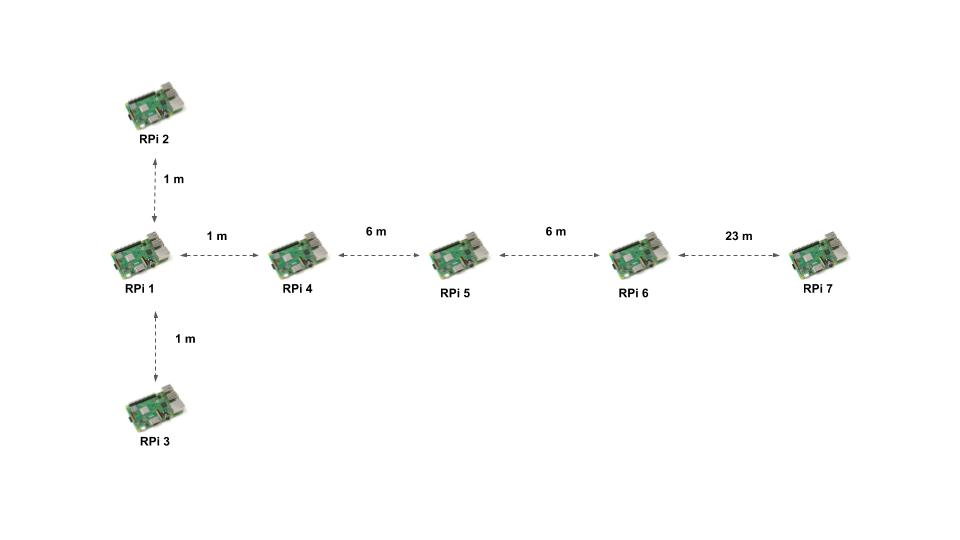
\includegraphics[width=6.5in]{images/devices_location.jpg}
\caption{Distance between each device in the factory environment.}
\label{fig_devices_loacation}
\end{figure}

\section{Adversary Model}
We assume a standard Dolev-Yao adversary model \cite{Dolev1981OriginalProtocols} where the adversary has complete control over all communication channels and it is not able to compromise the nodes. 
The adversary model considered for the design of a context-based authentication scheme is shown in Figure \ref{fig_environmentAttack}.
The model shows a network of devices located in the same environment, such as an office or in a delimited area in an industry, in which the devices are able to get the same ambient data such as light, audio and humidity. 
The goal of the adversary is to carry out relay attack by convincing the other nodes that it is nearby when in fact it is far away. 
The proposed countermeasure against relay attack which is based on the natural  assumption  that  two  entities  will  sense  similar ambient environments when they are co-present.
\begin{figure}[!h]
\centering
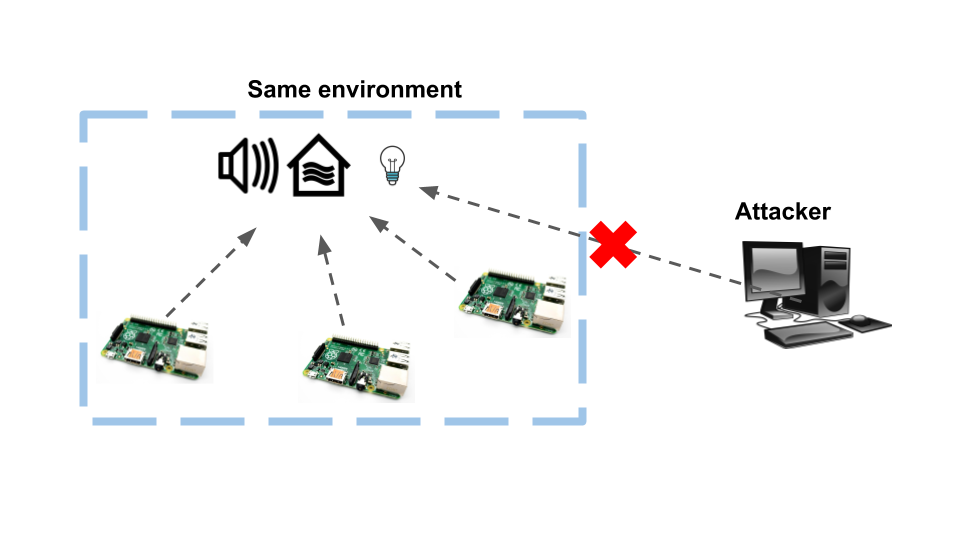
\includegraphics[width=5in]{images/environmentAttack.png}
\caption{For an attacker it is not possible to acquire the data from the user environment such as ambient sound, temperature and light.}
\label{fig_environmentAttack}
\end{figure}
    %%\chapter{Study Design}

    % $Id: methodology.tex 142 2012-12-22 10:41:32Z danbos $
\chapter{Implementation proximity-based authentication scheme}
\label{ch:implementationAuth}
This chapter describes the implementation and delineates the conducted work for the design of an authentication scheme based on context.

To be able to sense the ambient data, 
in Figure \ref{fig_device} is shown how the sensors used to collect the data are connected to the \acs{RPi}. 
\begin{figure}[!h]
\centering
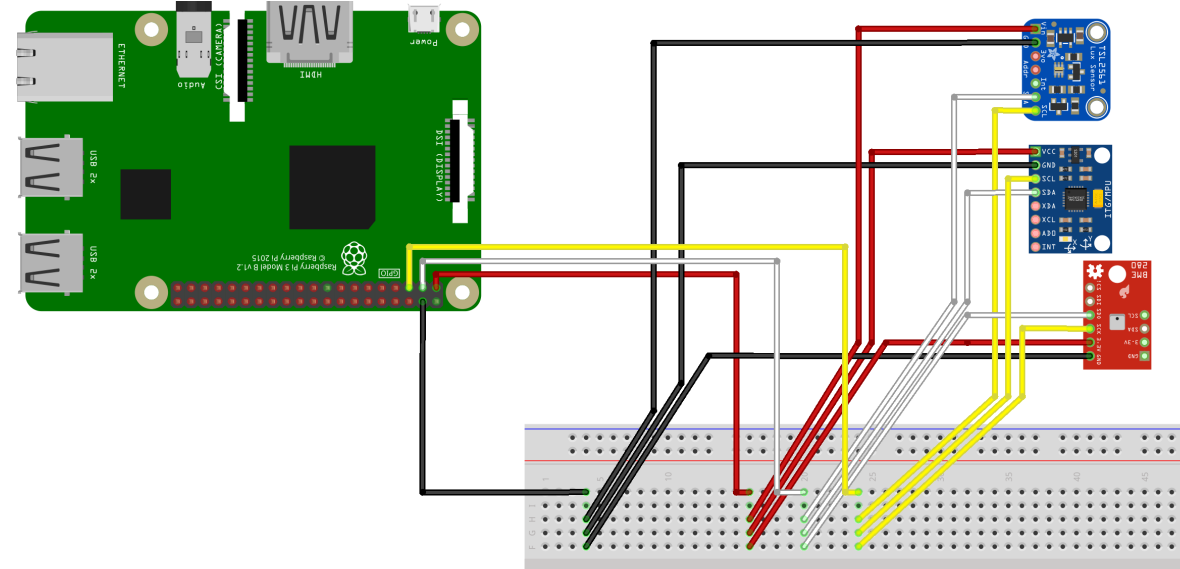
\includegraphics[width=6in]{images/device.png}
\caption{Raspberry Pi with the used context sensors.}
\label{fig_device}
\end{figure}

The  sensors direct digital output that can be sensed by the GPIO pins of the Raspberry Pi while the microphone is connected to the micro-controller through a USB sound card.
The system is using Raspbian as operating system which  is  the  massively  popular  OS for Raspberry Pi.
To get the data from the sensors have been used the following libraries:
\begin{itemize}
    \item{adafruit-circuitpython-bme280:} I2C and SPI driver for the Bosch BME280;
    \item{Adafruit\_CircuitPython\_TSL2591:} drivers for the sensors Adafruit TSL2591;
    \item{mpu6050-raspberrypi:} module for the sensor MPU6050;
\end{itemize}
The modules are all implemented in \textit{Python 3} which make easy to interact with them and to get the data.
To record audio has been used a script using the software \textit{ffmpeg} which allows the recording of audio through the sound card and its conversion to the \textit{.mp3} format in order to reduce their size.
The amount of RAM and computational power of the Raspberry  makes it commendable choice to get the real time data processed and accessed faster than other micro controller based systems.

The data sensing and the audio recording are started at the same time by a script and they save the data in file.
The tests have been executed for 24 hours, where has been constantly recorded the ambient audio and saved every 10 seconds the other ambient data.
To synchronize the start of the recording between the devices, a router has been used in order to connect them using wireless connection. 
From an external device has been sent a broadcast message to the devices connected and this triggers the start of the recording.

\section{Authentication protocol}
The authentication protocol has been implemented in $Python$ and is divided in two parts: fingerprint generation and fuzzy commitment scheme.

\subsection{Fingerprint}
The fingerprint extraction from the sensors function takes  the raw sensors data of length \textit{l\_sensor} values for each sensor and encode the signal to a fingerprint \textit{F} of length \textit{l\_F} bits. 
Two different fingerprint functions are implemented: one for the sensors and one for the audio.
\subsubsection{Fingerprint from sensor data}
The algorithm captures abrupt changes in the data and encodes them into high bits, mapping the remaining signal to low bits. 
The encoding algorithm is inspired from the one proposed in \cite{Nguyen2014Context-BasedDevices} and is divided in: 
\begin{itemize}
    \item \textbf{pre-processing:} apply a moving average filter to the raw data from each sensor. The raw data of a specific sensor are split in $k$ non overlapping segments of size $l\_segment$. A new vector $avg\_sensor$ is then generated by calculating the value's average of each segment.
    
    \item \textbf{generate fingerprint of each sensor:} we calculate each sensor data fingerprint as a sequence of bits $F_s$, in which each bit denotes the change of each $avg\_sensor$ value in comparison with the previous $avg\_sensor$ value. 
    The fingerprint bit corresponding to a value of $avg\_sensor$ is set to "1" if the relative change between two consecutive values of the vector $avg\_sensor$ is larger than a specified relative threshold $\Delta_r$ and if the difference between the values exceeds an absolute threshold value $\Delta_a$.
    In the other cases the bit is set to "0".
    \item \textbf{combine fingerprints:} the generated fingerprints $F_s$ are now concatenated in order to generate a unique context fingerprint \textit{F}. 
\end{itemize}

\subsubsection{Fingerprint from audio data}
The fingerprinting scheme is inspired by the one proposed in \cite{Schurmann2013SecureAudio}, where its security relies on the fact that the attacker is not sharing the context with the trusted devices.

In the proposed scheme, the devices start to record the sound for $t_s$ seconds generating an audio sequence $S$ with length $|S| = l_s = t_s \times r$, where $r$ is the sample rate.
The audio sequence is then split in $n_f$ frames  $S_1, \dots , S_n$ of length $|S_i| = d $ as shown in Figure \ref{fig_frames}.

\begin{figure}[!h]
\centering
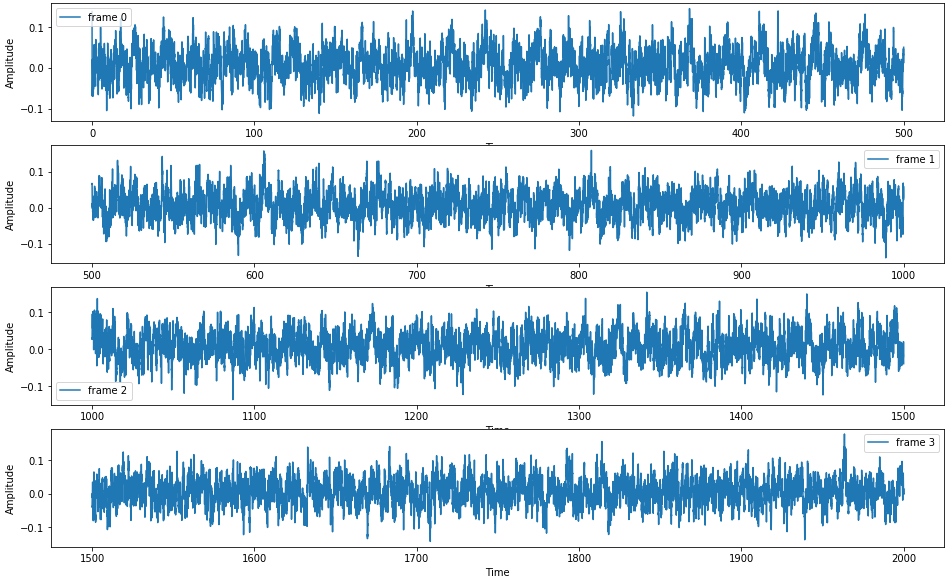
\includegraphics[width=6in]{images/frames.PNG}
\caption{Audio data split in frames. }
\label{fig_frames}
\end{figure}

On each frame is applied a discrete Fourier transformation (DTF) and calculated its absolute value (Figure \ref{fig_spectrums}):
\begin{center}
    $\forall i \in \{ 1, \dots , n \}$, 
    $FS_i = |DTF(S_i)|$
\end{center}

\begin{figure}[!h]
\centering
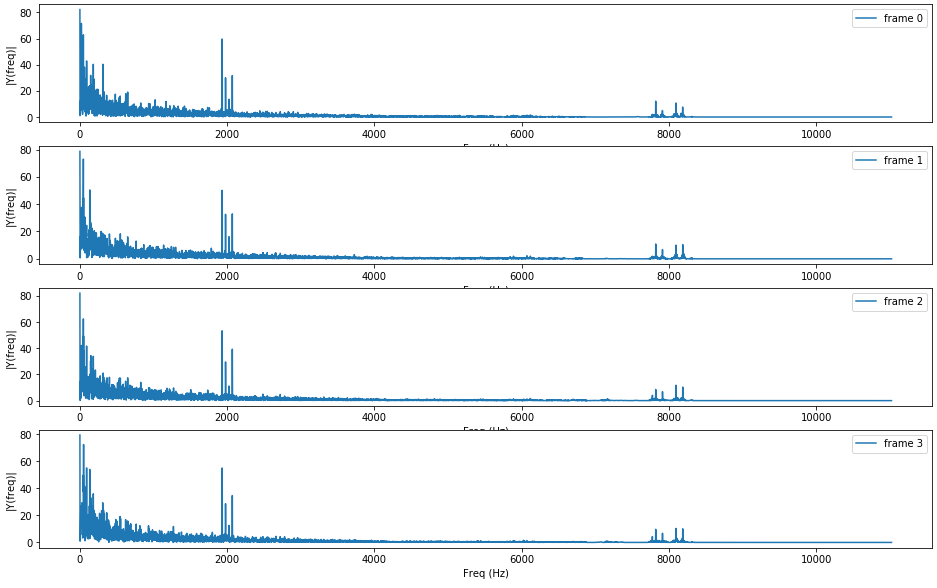
\includegraphics[width=6in]{images/spectrums.PNG}
\caption{Calculate the absolute value of the DTF on each frame. }
\label{fig_spectrums}
\end{figure}

Now the sets are summed together in order to to get a unique set of frequencies $FS_{tot}$ where the value  of the frequency $i$ is obtained by the sum of each val of $i$ of each set $S_i$.
Then a set $\overline{SF_{tot}}$ is obtained by applying an average filter of length $b$ over $FS_{tot}$ in order to remove noises as shown in Figure \ref{fig_spectrumsAVG}.

\begin{figure}[!h]
\centering
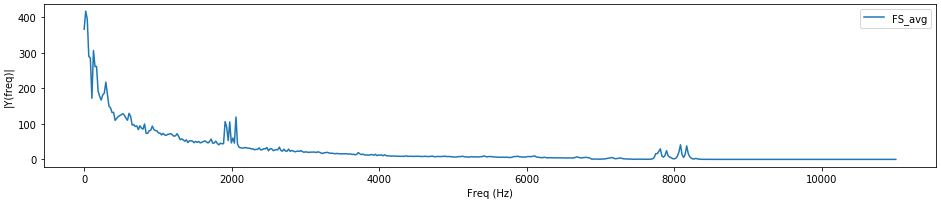
\includegraphics[width=6in]{images/spectrum_tot.PNG}
\caption{Generate $FS_{tot}$ and apply average  filter on it. }
\label{fig_spectrumsAVG}
\end{figure}

Based on the obtained sequence, it is possible to calculate the ambient audio fingerprint as a sequence of bits, in which each bit denotes the  change  of  the  $\overline{SF_{tot}}$  average value  in  comparison with  the  previous  $\overline{SF_{tot}}$'s  average.
The fingerprint bit corresponding to a value of $\overline{SF_{tot}}$ is set to "1" if the relative change between two consecutive values of the vector $\overline{SF_{tot}}$ is larger than a specified relative threshold $\Delta r_i$ and if the difference between the values exceeds an absolute threshold value $\Delta a_i$.
In the other cases the bit is set to "0".
$\Delta r$ and $\Delta a$ are two vector with the same dimension $|d_f|$ of the fingerprint and are generated by calculating the average of the relative changes  and absolute  differences between consecutive values in each frame $i \in \{0, \dots ,|d_f|-1 \}$ of $SF_{tot}$.

\subsection{Fuzzy commitment scheme}
For this part has been used the implementation proposed in \cite{fuzzyPairing}. 
This is a \textit{Python} implementation based on \cite{Juels2004AScheme} and it is divided in two main functions as shown in Figure \ref{fig_fuzzyCommit}: the commitment and the decommitment of a fuzzy commitment.
The commitment function is used to hide a randomly chosen set of bit $\kappa$ using the generated fingerprint $w$.
The decommitment method is designed in such a way that it receives a fingerprint $w'$ and if the Hamming distance is $Hamming(w , w') \leq t$ it can regenerate $\kappa$.

To implement these functions has been used a Reed-Solomon Python extension module based on the fast, GPL Reed-Solomon library by Phil Karn.
%%http://www.ka9q.net/code/fec/
The Reed-Solomon code $RS(q,m,n)$, with $q=2^k, k \in \mathbf{N} $ and $n <2^k$, is used to encode the random $\kappa$ to a codeword $c$ and to generate an "helper" value $\delta = c \oplus w$. 
During the decommitment phase, the Reed-Solomon scheme is used to decode a value $c' = w' \oplus \delta$ and get the value $\kappa$.
This procedure is capable of correcting up  to
\begin{center}
    $t = \dfrac{n - m }{2}$
\end{center}
differing  bits  between  the fingerprints.

\begin{figure}[!h]
\centering
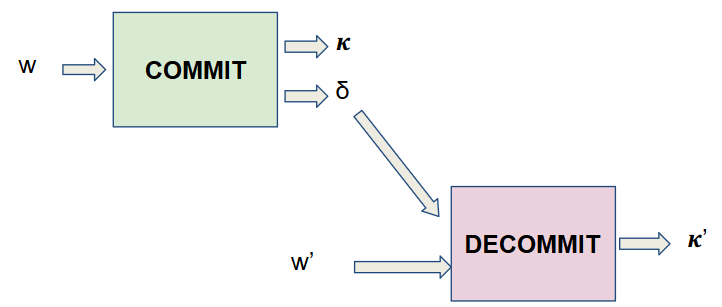
\includegraphics[width=4.5in]{images/fuzzy.PNG}
\caption{Fuzzy commitment scheme methods. }
\label{fig_fuzzyCommit}
\end{figure}
%    \chapter{Lightweight Group-Key Management}

It is fundamental to ensure security in network services and applications of WSNs and efficient and lightweight key management has been identified as one of core mechanisms to solve this problem.
In multicast group communications, the energy consumption, bandwidth and processing overhead at the nodes are minimized compared to a point-to-point communication system \cite{Rahman2015}. 
The multicast communication protocol has to generate and distribute a secret group key that can be used to encrypt data sent from one source to all destinations that are member of the same group. 
Multicast groups are often very dynamic due to the join and leave of the members, and for this reason the protocol has to handle such group membership changes by re-generating and re-distributing new group keys in a secure and efficient matter. 
Group key management in WSN includes several processes and mechanisms to solve the problem of  establishing a secure links between the members of a group.
This includes establishing (or creating), distributing and maintaining secret keys \cite{He2013JournalSurvey}.
The key establishment techniques should guarantee the authenticity of all the sensor nodes involved in a particular communication and protect the disclosure of data to unauthorized parties (i.e., confidentiality) and from falsifications (i.e. integrity).
Depending on the ability to update the cryptographic keys of sensor nodes during their run time (re-keying), these schemes can be classified into two different categories: static and dynamic.  
In static key management, the principle of pre-shared key is adopted, and keys are fixed for the whole lifetime  of  the  network.  
However, the probability for a cryptographic key to be attacked increases significantly with the time.  
Instead, in dynamic key management, the cryptographic keys are refreshed  throughout the lifetime of the network.

\section{Related Work}
%%%%% EDIT
This paper is based on a previous work presented in \cite{Gebremichael2018}.
There are well studied group key establishment protocols in use today. As described in \cite{Steiner1996}and \cite{Bresson2007}, it is possible to extend the Diffie-Hellman protocol to a group of nodes and generate a one-time session key. However, it is not ideal for power and resources constrained devices due to the intensive use of computational power. Moreover,it has been demonstrated that \cite{Bresson2007} do not meet some security requirements \cite{Bohli2007}.

A conference-key distribution system is proposed in \cite{Ingemarsson1982}. However it is demonstrated that the system is insecure because the information exchanged by the users makes it possible for a passive eavesdropper to compute the key. The approach used for \cite{Ingemarsson1982}  needs a high number of messages exchanged and executes an high number of integer exponentiation operations. %conference key distribution%

Some other protocols like $\mu$TESLA \cite{Perrig2002} are some of the earliest proposed protocols in the category symmetric key based protocols and they are based on hash function to reduce the energy consumption but they do not check for data integrity. Other symmetric key schemes based on key ring like \cite{Bohli2007} are not scalable, and therefore, these are unsuitable for dynamic environments such in our scenario.

In \cite{Porambage2015} the authors propose two lightweight group-key establishment protocols using an approach similar to ours.
The first protocol allows only the legitimate members of the multicast group as eligible to continue the rest of the process of key derivation. 
This one is more appropriate for distributed IoT applications, which require nodes to contribute hightly to the key computation and need greater randomness. 
The second one allows to establish a shared secret key among the multicast group. This one is more suitable for centralized IoT applications, where a central entity performs the  majority of the cryptographic functions. 

    \chapter{Lightweight Group-Key Management Scheme}
\label{ch:lightwightProto}
It is fundamental to ensure security in network services and applications of WSNs and efficient and lightweight key management has been identified as one of core mechanisms to solve this problem.
In multicast group communications, the energy consumption, bandwidth and processing overhead at the nodes are minimized compared to a point-to-point communication system \cite{Rahman2015}. 
The multicast communication protocol has to generate and distribute a secret group key that can be used to encrypt data sent from one source to all destinations that are member of the same group. 
Multicast groups are often very dynamic due to the join and leave of the members, and for this reason the protocol has to handle such group membership changes by re-generating and re-distributing new group keys in a secure and efficient matter. 

Group key management in WSN includes several processes and mechanisms to solve the problem of  establishing a secure links between the members of a group.
This includes establishing (or creating), distributing and maintaining secret keys \cite{He2013JournalSurvey}.
The key establishment techniques should guarantee the authenticity of all the sensor nodes involved in a particular communication and protect the disclosure of data to unauthorized parties (i.e., confidentiality) and from falsifications (i.e. integrity).

Depending on the ability to update the cryptographic keys of sensor nodes during their run time (re-keying), these schemes can be classified into two different categories: static and dynamic.  
In static key management, the principle of pre-shared key is adopted, and keys are fixed for the whole lifetime  of  the  network.  
However, the probability for a cryptographic key to be attacked increases significantly with the time.  
Instead, in dynamic key management, the cryptographic keys are refreshed  throughout the lifetime of the network.

The proposed protocol focuses on different problems related to group-key establishment and management.

First, is considered the problem of establishing a group shared secret among a group of end nodes. 
Then the author shows how a new node can be added to the group in such a way that the newly added node does not learn the previous group key or group communication. 
It is also shown how to remove a node from the group in such a way that it does not learn anything about the communications after it left the group. 
Finally, the problem of generating new session keys from the established group secret is analyzed.  

In this thesis, it has been adopted a slightly loose definition of forward and backward secrecy. 
By forward secrecy, the author means that an attacker will not able to learn future session keys or group communications even if the attacker managed to learn the current session key.
This also applies to which was a member of the group but that was later removed. 
Even that node had access to the session key when it was a member, it shall not be able to learn or derive session keys generated after it left the group. 
By backward secrecy, it is meant that a newly added node will not be able to learn previous session keys and/or group communication before it joined the group. 

\begin{table}[h]
\caption{List of Notations for the proposed scheme }
\label{notations}
\begin{center}
\begin{tabular}{|c||c|}
\hline
\textbf{Notation} & \textbf{Description}\\
\hline
\textit{G} & Gateway\\
\hline
$n_i$ & $i$th node\\
\hline
$k$ & number of nodes\\
\hline
$m$ & number of legitimate nodes\\
\hline
$PrivKey_i$ & $i$th node's private key\\
\hline
$PubKey$ & $i$th node's public key \\
\hline
$\mathbb{F}_q$ & finite field\\
\hline
$\mathbb{E}|\mathbb{F}_q$ & elliptic curve on the finite field $\mathbb{F}_q$\\
\hline
$s_i$ & secret shared between $i$th node and the gateway \\
\hline
E & generic symmetric encryption/decryption function (i.e, AES) \\
\hline
$MSK$ & final group shared secret (Master Shared Key) \\
\hline
$PRF$ & Pseudo Random Function \\
\hline
\end{tabular}
\end{center}
\end{table}

\section{Initialization Procedure}

\tikzstyle{drawrect}=[draw, rectangle,anchor=east, minimum height=8,
  minimum width=142pt,fill=Turquoise!20]
\begin{figure*}
\begin{center}
\begin{tikzpicture}[auto,rotate=90,transform shape]
    \draw (-8,0) -- (-8,-13)[dashed] (-1,0) -- (-1,-13)  (4.5,0) -- (4.5,-13)  (10,0) -- (10,-13);
    \node at (-8,.3) [draw,thin]{\textbf{Gateway}};
    \node at (-1,.3) [draw,thin]{\textbf{Node 1}};
    \node at (4.5,.3) [draw,thin]{\textbf{Node 2}};
    \node at (10,.3) [draw,thin]{\textbf{Node 3}};
    \node at (-8.25,-2) [drawrect, rotate=90, fill= SkyBlue!5, minimum width=7cm]  { Timeout};
    \draw[->, dashed, draw=red] (-8,-2) -- node[midway,above,align=left] {
        \small Broadcast: "\textit{New Group}",\\$group\_ID, \delta , PubKey$ 
        } (-2,-2);
    \draw[<-] (-8,-4) -- node[midway,above,align=left] {
    $\bullet$ \small calculate  $s_1$ and  $\kappa_1 = f(x_1,\delta)$\\
    $\bullet$ \small HMAC($\kappa_1 , s_1$)\\
    $\bullet$ \small $PubKey_1$
    } (-1,-4);
    
    \draw[<-] (-8,-6) -- node[midway,above,align=left] {
    $\bullet$ \small calculate  $s_2$ and  $\kappa_2 = f(x_2,\delta)$\\
    $\bullet$ \small HMAC($\kappa_2 , s_2$)\\
    $\bullet$ \small $PubKey_2$
    } (4.5,-6);
    
    \draw[<-] (-8,-8) -- node[midway,above,align=left] {
    $\bullet$ \small calculate  $s_3$ and  $\kappa_3 = f(x_3,\delta)$\\
    $\bullet$ \small HMAC($\kappa_3 , s_3$)\\
    $\bullet$ \small $PubKey_3$
    } (10,-8);
    
    \draw[->] (-8,-10) -- node[midway,above,align=left] {
    $\bullet$ \small Compute secrets $s_1, s_2, s_3$ \\
    \small Compute $group\_secret = s_1 \times s_2 \times s_3$ \\
    $\bullet$ \small encrypt ($partial\_secret = s_2 \times s_3$)
    } (-1,-10);
    
    \draw[->] (-8,-11.5) -- node[midway,above,align=left] {
    $\bullet$ \small encrypt ($partial\_secret = s_1 \times s_3$)
    } (4.5,-11.5);
    
    \draw[->] (-8,-12.5) -- node[midway,above,align=left] {
    $\bullet$ \small encrypt ($partial\_secret = s_1 \times s_2$)
    } (10,-12.5);
    
    \node at (-1,-13.5) [draw,thin, align=left, anchor=east, fill= SkyBlue!5 ]{
    \small $\bullet$ $group\_secret = s_1 (s_2 s_3)$\\
    \small$\bullet$ $MSK = group\_secret  \times \mathbb{P}$};
    
    \node at (4.5,-13.5) [draw,thin, align=left, anchor=east, fill= SkyBlue!5 ]{
    \small$\bullet$ $group\_secret = s_2 (s_1 s_3)$\\
    \small $\bullet$ $MSK = group\_secret  \times \mathbb{P}$};
    
    \node at (10,-13.5) [draw,thin, align=left, anchor=east, fill= SkyBlue!5 ]{
    \small$\bullet$ $group\_secret = s_3 (s_1 s_2)$\\
    \small$\bullet$ $MSK = group\_secret \times \mathbb{P}$};
\end{tikzpicture}
\end{center}
\caption{Group Key Initialization: The figure shows the messages exchanged between G and three end nodes which replied to the join request before the
specified timeout.}
\label{fig_group_key}
\end{figure*}

In this phase, a device that wants to start a secure group, usually the gateway, generates a unique $group\_ID$ and includes it in a "\textit{new\_group}" broadcasts message.
It also generate a public key $PubKey$ represented as a point on an elliptic curve and a couple of values $(\h(\kappa), \delta)$ through a commitment function $F$ using a context fingerprint as described in \ref{proxAuth}, including them in the broadcast message.

Now a specified timeout starts and the nodes that want to join the group reply to the broadcast message with their public key $PubKey_i$ in a \textit{JOIN} message. 
Each node calculate a secret $s_i$ shared with the gateway generated with Elliptic-curve Diffie-Hellman (\acs{ECDH}) protocol and , using a decommitment function $f$, extract from their context fingerprint $x_i$ the value $\kappa_i = f(x_i, \delta)$.
In the message, together with its public key, each node $i$ include the value $HMAC(\kappa_i, s_i)$, in order to guarantee confidentiality and authenticity.

The gateway \textit{G} collects the \textit{JOIN} replies until the timeout expires and then it calculates the secrets shared with each node $i$ willing to join the group and checks that $HMAC(\kappa , s_i) = HMAC(\kappa_i, s_i)$ in order to verify both integrity of the received message and that the node is located in the same ambient.
\textit{G} computes the $group\_secret = \prod_{i=1}^{m} s_{i}$ where $m$ is the number of nodes which replied to the $JOIN$ message and have been authenticated. \textit{G} finally sends to each node $n_i$ the value $partial\_secret = group\_secret / s_i$, encrypted with the shared secret using protocols such as AES.
This procedure is shown in Algorithm \ref{alg:init}.

\begin{algorithm}
\caption{Group-key initialization }\label{alg:init}
\hspace*{\algorithmicindent} \textbf{Input:} parameter $\mathbb{P}$ \\
\hspace*{\algorithmicindent} \textbf{Output:} \textit{group\_secret} \\
\hspace*{\algorithmicindent} \textbf{Initialization:} chose $group\_id, group\_secret = 1$, \\
\hspace*{\algorithmicindent} Broadcast group join request with {\textit{group\_id}, $\delta$, $PubKey$ }\\
\hspace*{\algorithmicindent} Set \textit{timeout}
\begin{algorithmic}[1]
\While{$timeout$ not expired}
\For{for each $JOIN_i$ message received} 
\State generate shared secret $s_i$
\If{$HMAC(\kappa, s_i) == HMAC(\kappa_i , s_i)$}
\State $group\_secret = group\_secret * s_i$
\EndIf
\EndFor{}
\EndWhile\label{secret}
\For{for each $s_i$ received and validated} 
\State $G \rightarrow n_i: \qquad E_{s_i}(group\_secret / s_i)$
\EndFor{}
\Return{$group\_secret$}
\end{algorithmic}
\end{algorithm}

After receiving the message, each node $n_i$ decrypts the message obtaining its own $partial\_secret$ and computes  
\begin{center}
$MSK = partial\_secret * s_i * \mathbb{P}$
\end{center}
where $MSK$ represents the group shared key.

\section{Join Procedure}
After establishing a secure $group\_secret$, the addition of a new node in the group may occur. 
When a new node $new\_node$ wants to join the group, it sends a message to $G$ containing the $group\_ID$ and its public key $PubKey$.
The gateway generate a couple of values $(\h(\kappa), \delta)$ through a commitment function $F$ using a fingerprint of its context and sending a \textit{challenge} to the $new\_node$ with a message containing $\delta$ and its own public key $PubKey$.
The new node replies to the the challenge with $HMAC(\kappa_n, s_n)$, where $\kappa_n$ is the secret key generated using a commitment function $F$ exploiting a context fingerprint.
At this point $G$ can verify that $new\_node$ is located in the same ambient and recomputes the $group\_secret$ as before including the secrets from the new nodes and broadcasting the $new\_MSK = group\_secret \times P$, encrypting the message with the previous $MSK$. 

In this phase we have to ensure that the new node isn't able to easily recover the old $MSK$. 
To solve this problem, $G$ picks a random secret $s_i$ from the nodes already present in the group  and sends to the $new\_node$ a message, encrypted with his shared secret $s_n$, containing $s_{i}\mathbb{P}$ and $partial\_secret = new\_group\_secret / s_i$.

\begin{algorithm}[H]
\caption{New node addition }\label{alg:newNode}
\hspace*{\algorithmicindent} \textbf{Input:} parameter $\mathbb{P}$ \\
\hspace*{\algorithmicindent} \textbf{Output:} \textit{group\_secret} \\
\hspace*{\algorithmicindent} \textbf{Initialization:} chose the \textit{group\_id} of the group to join,\\
\begin{algorithmic}[1]
\State $new\_node \rightarrow G:\qquad group\_ID, PubKey_n$
\State $G \rightarrow new\_node:\qquad \delta, PubKey$
\State $new\_node \rightarrow G:\qquad HMAC(\kappa_n, s_n)$
\If{$HMAC(\kappa_n, s_n) == HMAC(\kappa, s_n)$}
\State $old\_MSK = MSK$
\State $group\_secret = s_n * old\_group\_secret$
\For{for each node $n_i$ already in the group} 
\State $G \rightarrow n_i: \qquad E_{old\_MSK}( (MSK / s_i) \times \mathbb{P})$
\EndFor{}
\State $G$ picks a random $s_i$ of a node already in the group
\State $partial\_secret = group\_secret / s_i$
\State $G \rightarrow new\_node: \qquad E_{s_n}(s_{i}\mathbb{P}, partial\_secret)$
\State $new\_node$ calculates $MSK = s_{i}\mathbb{P} \times partial\_secret$\\
\EndIf
\Return{$group\_secret$}
\end{algorithmic}
\end{algorithm}

To obtain the $MSK$, the new node only has to multiply $s_{i}\mathbb{P}$ by $partial\_secret$ and it will not be able to recover the old $MSK$ due to difficulty to obtain $s_i$ from $s_{i}\mathbb{P}$.  %mention why it is difficult ? %
This procedure is shown in Algorithm \ref{alg:newNode}.

\section{Leave Procedure}

\begin{algorithm}[H]
\caption{Node removal's algorithm }\label{alg:remNode}
\hspace*{\algorithmicindent} \textbf{Input:} parameter $\mathbb{P}$ \\
\hspace*{\algorithmicindent} \textbf{Output:} \textit{group\_secret} \\
\hspace*{\algorithmicindent} \textbf{Initialization:} remove the node $n$ from the \\
\hspace*{\algorithmicindent} group $group\_id$\\
\begin{algorithmic}[1]
\State $G$ picks a random $s$ of a node in the group
\State $partial\_secret_i = group\_secret / (s_i s)$
\For{for each node $n_i$ already in the group} 
\State $G \rightarrow n_i: \qquad partial\_secret_i , s \mathbb{P}$
\EndFor{}

\State $n_i$ calculates $MSK = s \mathbb{P} * partial\_secret_i$\\
\Return{$group\_secret$}
\end{algorithmic}
\end{algorithm}

It can happen that one or more nodes have to be removed from the group for various reasons. In such an event, the protocol has to ensure forward secrecy of the $MSK$ to avoid the possibility that the removed node is able to get the new group secret. 
The gateway proceeds as described before picking up a random node's shared secret $s$ and sends to each node $n_i$ which belongs to the group a message containing a new partial secret $partial\_secret_i = group\_secret / (s_i s)$ and $s\mathbb{P}$. 
Each node can than compute $MSK$ by multiplying $partial\_secret_i$ by $s\mathbb{P}$ and its shared secret $s_i$. 
The nodes that have left the group will not be able to compute the new $MSK$ due to the same reason described during the \textit{node addition´s phase}.

\section{Generate Session Key}
After the $MSK$ generation, it is possible to use symmetric key encryption to encrypt the group messages. The choice of using symmetric key encryption instead of public key encryption is motivated by the fact that public key encryption is slower and requires more computation power, a critical point in this class of constrained IoT devices. 

Using the same key for more than one session makes the protocol vulnerable to many attacks \cite{Syverson}, so we generate new and pseudorandom keys from the $MSK$. The session key can be produced and managed in different ways depending on whether the encryption scheme is block or stream cipher. In this section we consider those two methods separately.  
$MSK$ with block ciphers: Suppose the block cipher of our
choice takes n-bit key size. Therefore, every session key must
be n-bit long. We assume we have a k-bit output hash function
h, and a $PRF$ that maps an input of l-bit key size to an output
of size $n$. Note that the output of the $PRF$ is computationally
indistinguishable from an output of a random function from
l to n. An l-bit input seed to our $PRF$ is first formed by
concatenating the results of a repeated application of a hash
function applied to a nonce and $MSK$, as shown below.
\begin{center}
$seed = h(nonce_1 \parallel MSK) \parallel h(nonce_2 \parallel MSK) \parallel \cdots$
\end{center}
A session key is then generated by feeding the seed into a
$PRF$.
\begin{center}
$session\_key = PRF(seed)$
\end{center}
And finally $MSK$ is updated to the new session key. 
Note that the node sending a group message randomly selects as many nonce values as needed to create an l-bit output. 
The nonce values are sent in the clear to all nodes so that every nodes updates its session key similarly.

$MSK$ with stream ciphers: in this case, it is required tha twe produce a session key as long as the length of the text
to be encrypted. This can be achieved by concatenating the
results of the $PRF$ on many seed values as follows.
\begin{center}
$seed 1 = h(nonce_1 \parallel MSK)$\\
$seed_2= h(nonce_2 \parallel MSK)$\\
$\vdots$ \\
$seed_n = h(nonce_n \parallel MSK)$
\end{center}

We then apply the $PRF$ to each seed seed and simply
concatenate the results to generate a session key as long as
required.
\begin{center}
$session\_key = PRF (seed_1) || PRF (seed_2) || \cdot$
\end{center}
In both cases, encryption is done as follows :
\begin{center}
$Encrypt(M) = f(M, Session key)$
\end{center}
Where $f$ could by any block cipher, such as AES, or stream
cipher, such as RC4.


	\chapter{Implementation of the Lightweight Protocol}
\label{ch:implementationProto}
\section{Implementation Environment}
\subsection{Operating System}
To check the feasibility and analyze the performances, the proposed  framework has been  implemented on  the  Contiki OS and measured its performance using the COOJA simulator\cite{Osterlind2006}.  
Contiki provides the whole development environment( including compilers and development tools ) in an Ubuntu virtual machine called Instant Contiki.
In this thesis has been used Instant Contiki 3.0, released on August 25, 2015. 
COOJA  is  a  network  simulator  that  allows  the  simulation  of  IoT  resource-constrained  networks. 
COOJA allows to test the code and systems before running it on the target hardware or also referred as mote, verifying then its behavior.
It also  offers  an interface that can be used to analyze the messages exchanged in  the  network  during  protocol  execution  and  calculate  the energy  consumption  and  execution  time Contiki  Energest.

\subsection{Tmote Sky}
In this study we simulate Tmote Sky node over an MSP430 microcontroller \footnote{https://insense.cs.st-andrews.ac.uk/files/2013/04/tmote-sky-datasheet.pdf} based board.
Tmote Sky is a low power wireless sensor with integrated humidity, temperature, and light sensors;
its details are shown in Table \ref{tmote}.
\begin{table}[H]
\caption{The main characteristics of the Tmote sky}
\label{tmote}
\begin{center}
\begin{tabular}{|c||c|}
\hline
\bf Resource & \\
\hline
Operating Voltage & 3 V\\
\hline
Microcontroller & (16 bit)8 MHz\\
\hline
RAM & 10 KB\\
\hline
ROM & 48 KB\\
\hline
Low Power Mode (LPM) & 0.0545 mA\\
\hline
Current consumption TX mode & 19.5 mA\\
\hline
Current consumption RX mode & 21.8 mA\\
\hline
Ticks/second & 327680\\
\hline
\end{tabular}
\end{center}
\end{table}

Tmote Sky corresponds to \textit{Class 1} devices according to the terminology for constrained-node networks \cite{Bennett2014TerminologyNetworks} and is our choice since it is well known, widely used, and supported by Cooja.
Tmote Sky does not have support for cryptographic operation needed by the proposed protocol as the only cryptographic operation supported by cc2420 radio chip is AES-128 encryption.
%\subsubsection{Sensors}
%Mini USB Microphone https://www.m.nu/ljud/mini-usb-microphone
%QWIIC ENVIRONMENTAL COMBO BRKOUT  %https://www.digikey.se/product-detail/en/sparkfun-electronics/SEN-14348/1568-1706-ND/7652735?utm_adgroup=Expansion+Boards&mkwid=s&pcrid=260389032456&pkw=&pmt=&pdv=c&productid=7652735&slid=&gclid=EAIaIQobChMIp47_wKjZ4AIVxKiaCh3RtQKREAQYASABEgKK7fD_BwE

\section{Network Configuration}
It is defined as multicast group a particular group of nodes, which are entitled to receive the common set of information.
In  this  thesis,  we  consider  a  network  composed  by  a  set \textit{G} of nodes connected to a gateway \textit{GW} as shown in Figure \ref{fig_network}

\begin{figure}[!h]
\centering
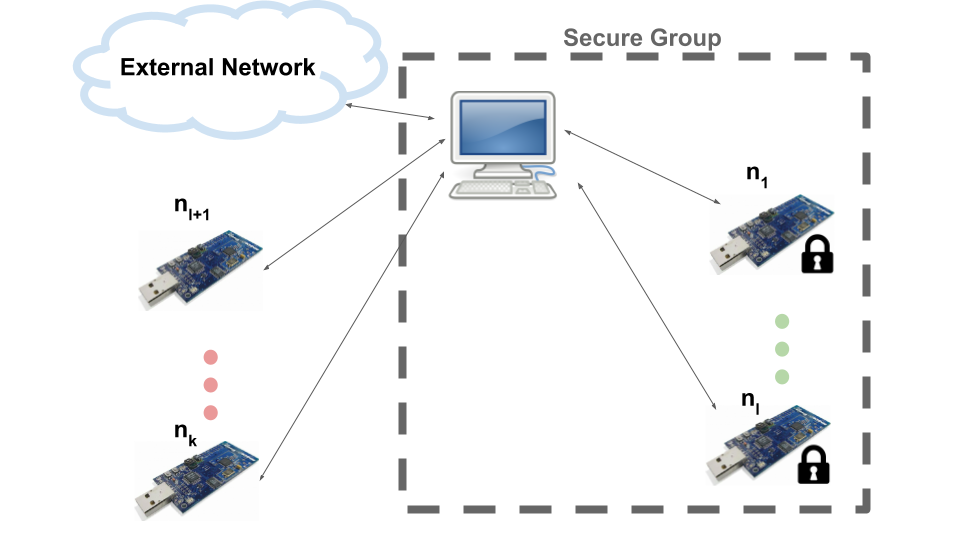
\includegraphics[width=5in]{images/network2.png}
\caption{Network Model. The network consists of a gateway and a set of nodes, supported by a communication infrastructure. All or a part of the nodes may be members of a group as shown in the figure (m nodes are in the group).}
\label{fig_network}
\end{figure}
Formally, the network can be modeled as a graph $Gr = \langle GW, N, E\rangle$ where \textit{GW} is the gateway that acts as a group initiator and manager and \textit{N} is a set of nodes $n_1, n_2, \dots, n_k$, and \textit{E} is the set of edges from \textit{GW} to $n_i$ representing bi-directional communication links.

\textit{GW} is considered a trustworthy entity which acts as  the group-manager which includes creating new groups, adding new nodes to the groups and maintaining the keys and the members of nodes of each group.
The gateway can be implemented according to a distributed architecture, providing benefits in terms of availability and robustness, avoiding to have a single point of failure on the single instance \textit{GW}.

It is also assumed that this communication technology and sensor nodes support  the transaction of multicast messages and is considered that all the entities in the network possess the same security associations and perform identical cryptographic functions. In our specific tests the entities support the following security functionality:
\begin{itemize}
\item Symmetric encryption scheme, specifically \acs{AES};
\item \acs{HMAC} function;
\item Hash functions, specifically SHA2.
\end{itemize}

\section{Code Implementation}
The proposed protocol consists of 2 important components: the nodes and the gateway.

The gateway and the nodes uses cryptographic operations: the decryption / encryption with AES, elliptic curve point multiplication and HMAC. As mentioned before, Tmote Sky has no support in hardware level for those cryptographic operations used by the proposed protocol. Thus, those cryptographic operations are implemented in application level using some existing C code examples with some modifications. As the consequence, the nodes and gateway memory occupancy and computing time may be higher compared to the case if the sensor supports those cryptographic functions in hardware level.

The module performing the basic elliptic curve point operations such as multiplication and addition is a C implementation based on $kmackay$'s $micro-ecc$.
This module include the ECDH and ECDSA functions and is an implementation for 8-bit microcontrollers.%%% CITATION https://github.com/iSECPartners/nano-ecc

For the implementation of the AES encryption algorithms with keys 192-bit long has been used a C implementation. %%%%%%%CITATION https://github.com/kokke/tiny-AES-c
The original module occupies relatively small memory and suitable for devices with little endian format.

The HMAC module is Software implementation in C of the FIPS 198 Keyed-Hash Message Authentication Code for SHA2 .
%%%%CITATION https://github.com/ogay/hmac

For the communication between the devices has been used the Rime communication stack. %CITATION RIME
Rime is a lightweight layered communication  stack for sensor networks created to simplify implementation of sensor network  protocols and facilitate code reuse.
Rime is already implemented in Instant Contiki 3.0 and has code footprint less than two kilobytes, with data memory requirements on the order of tens of bytes.


At the node's startup, a pair of private and public keys is generated and it start listening to broadcast connection to port 129. After receiving the Broadcast message from the gateway, each node start to listen on the port $146$ for unicast messages instead.


\begin{table}[H]
\caption{Node and Gateway Memory Usage [bytes] }
\label{nodeUsage}
\begin{center}
\begin{tabular}{|c|c|c|c|c|c|}
\hline
\textbf{Device} & \textbf{Text} &\textbf{Data} & \textbf{bss} & \textbf{dec} & \textbf{hex}  \\
\hline
Node & 26821 & 302 & 5524 & 32647 & 7f87\\
\hline
Gateway & 28077 & 302 & 5634 & 34013 & 84dd\\
\hline
\end{tabular}
\end{center}
\end{table}

In Table \ref{nodeUsage} we show the memory usage of the node and the gateway in bytes. 
\textit{text} shows the size of the code section in bytes (this will typically be in ROM).
\textit{data} and \textit{bss} show sections that contain variables, stored in RAM. 



	%\chapter{Evaluation}
\label{ch:evaluation}
This chapter outlines the depicted scenario and describes the approach applied in this thesis project work. Further, a section is devoted to each the utilized settings, the used hardware, and the software libraries applied for the conducted thesis project work.




These are example section titles! Choose to your own needs


\section{Scenario}


\section{Approach}

%\begin{figure}[H]
%\centering
%\includegraphics[width=0.95\textwidth]{img/approach_v1.png}
%\caption{The figure shows a visual representation of the approach pursued in this master thesis work. A detailed view %of Figure \ref{fig:overviewimpl} is shown where the link-up of the sensing platform and the fog computing node is %visualized.}
%\label{fig:approach}
%\end{figure}


\section{Settings}


\section{Hardware}

\section{Software}

	\chapter{Results} 
\label{ch:results}
This chapter presents and describes the results of the conducted performance evaluation of the context-based authentication protocol and group-key management protocol. 

\section{Performances of the authentication scheme}
In this project two different fingerprints are proposed: one based on the ambient data from the sensors and one based on the recorded audio.
The similarity of these fingerprints is then used to decide if devices can establish a connection by using a key generated from fuzzy commitment scheme.

The fingerprint length generated from the ambient data is 320 bits long and required 1000 data from each sensor, which means that the device has to acquire data for 10000 seconds.
The features used to generate this fingerprint are: temperature, humidity, gas, light and  pressure.
For the analysis have been used only the parameters which were correlated among the devices during the time and the ones obtained from the gyroscope and accelerometer were completely discorrelated.
A fingerprint 64-bit long is generated from each feature and then they have been combined in order to generated a unique 320 bit long fingerprint.

The fingerprint generated from the recorded audio has a length of 512 bits and required 10 seconds of audio recording.
In Table \ref{tab_sensorAcc} and Table \ref{tab_audioAcc} are shown the performances of the two fingerprints while changing the number of different bits $t$ between 2 different fingerprints.

The analysis is performed comparing fingerprints from the same environment but in different times in order to verify if the scheme is able to identify if two fingerprints are generated in different periods.
In the tables are shown the following parameters: 
\begin{itemize}
    \item the amount of authenticated true claims (T.A.) 
    \item the amount of not authenticated false claims (T.R.)
    \item the amount of authenticated false claims (F.A.)
    \item the amount of not authenticated true claims(F.R.)
\end{itemize}

\begin{table}[H]
\label{tab_sensorAcc}
\begin{center}
\begin{tabular}{|c|c|c c c c|}
\hline
&\multicolumn{5}{c|}{\textbf{Sensors}} \\\cline{2-6}
\textbf{Environment} & \textit{t} &\textbf{T.A.}& \textbf{T.R.} & \textbf{F.A.}& \textbf{F.R.} \\ \cline{1-6}
\multirow{4}{*}{Factory}
& 50 & 1 & 1071 & 0 & 104 \\ \cline{2-6}
& 80 & 18 & 1065 & 6 & 87 \\ \cline{2-6}
& 92 & 46 & 1059 & 12 & 70 \\ \cline{2-6}
& 100 & 55 & 1055 & 16 & 50 \\ \cline{1-6}
\multirow{4}{*}{Lab}
& 50 & 0 & 525 & 0 & 70 \\ \cline{2-6}
& 80 & 5 & 525 & 0 & 65 \\ \cline{2-6}
& 92 & 20 & 525 & 0 & 50 \\ \cline{2-6}
& 100 & 36 & 519 & 6 & 34 \\ \cline{1-6}
\end{tabular}
\caption{Accuracy results of the fingerprints generated from the sensors data changing the parameter $t$.  }
\end{center}
\end{table}

\begin{table}[H]
\label{tab_audioAcc}
\begin{center}
\begin{tabular}{|c|c|c c c c|}
\hline
&\multicolumn{5}{c|}{\textbf{Audio}} \\\cline{2-6}
\textbf{Environment} & \textit{t} &\textbf{T.A.}& \textbf{T.R.} & \textbf{F.A.}& \textbf{F.R.} \\ \cline{1-6}
\multirow{4}{*}{Factory}
& 190 & 54 & 151 & 369 & 21 \\ \cline{2-6}
& 180 & 39 & 254 & 266 & 36 \\ \cline{2-6}
& 170 & 16 & 362 & 158 & 59 \\ \cline{2-6}
& 160 & 6 & 434 & 86 & 69 \\ \cline{1-6}
\multirow{4}{*}{Lab}
& 180 & 9 & 12 & 238 & 1 \\ \cline{2-6}
& 170 & 44 & 44 & 206 & 6 \\ \cline{2-6}
& 160 & 32 & 82 & 168 & 18 \\ \cline{2-6}
& 150 & 18 & 123 & 127 & 32 \\ \cline{1-6}
\end{tabular}
\caption{Accuracy results of the fingerprints generated from the recorded audio changing the parameter $t$. }
\end{center}
\end{table}

In the factory's use case, the device  located far from the others is considered in a different environment.
The results show how difficult is to recognize fingerprints generated in different time periods. 
In Table \ref{tab_rejectionAudio} and Table \ref{tab_rejectionSensor} has been applied the fuzzy commitment scheme between devices located in different environments.
The tests are performed changing the parameter $t$ used by the error correcting code scheme.

The results show that when two devices are located in different environments, they produce dissimilar fingerprints and even with high values of $t$, it results difficult to authenticate them.
In fact, using an error correcting code able to correct the 35 \% of the message in the case of audio fingerprints and 37\% in the case of the fingerprint generated by the other ambient features, the scheme authenticate devices in different environments the 13.3 \% and 12.3\% of the cases respectively.

\begin{table}[H]
\label{tab_rejectionSensor}
\begin{center}
\begin{tabular}{|c|c c c|}
\hline
\multicolumn{4}{|c|}{\textbf{Sensors}} \\\hline
\textit{t} &\textbf{False Authenticated}& \textbf{True Rejected}& \textbf{Error Rate (\%)}  \\ \cline{1-4}
130 & 534 & 1181 & 31.1\\ \cline{2-4}
120 & 211 & 1504 & 12.3\\ \cline{2-4}
110 & 60 & 1655 & 3.5\\ \cline{2-4}
100 & 12 & 1703 & 0.7\\ \cline{2-4}
90 & 0 & 1715 & 0 \\ \cline{1-4}
\end{tabular}
\caption{Authentication using fingerprints generated from the sensors data by devices located in different environments. }
\end{center}
\end{table}

\begin{table}[H]
\label{tab_rejectionAudio}
\begin{center}
\begin{tabular}{|c|c c c|}
\hline
\multicolumn{4}{|c|}{\textbf{Audio}} \\\hline
\textit{t} &\textbf{False Authenticated}& \textbf{True Rejected}& \textbf{Error Rate (\%)}  \\ \cline{1-4}
180 & 116 & 759 & 13.3\\ \cline{2-4}
170 & 75 & 800 & 8.6\\ \cline{2-4}
160 & 49 & 826 & 5.6\\ \cline{2-4}
150 & 20 & 855 & 2.3\\ \cline{2-4}
140 & 4 & 871 & 0.5\\ \cline{2-4}
130 & 0 & 875 & 0\\ \cline{1-4}
\end{tabular}
\caption{Authentication using fingerprints generated from the recorded audio by devices located in different environments. }
\end{center}
\end{table}

\section{Lightweight protocol}
 In this section is presented the performance results of the proposed scheme comparing it with the scheme designed in \cite{Porambage2015}
In order to perform the performance evaluation, the environment is set.
The evaluation is done for a sensor network consists of 5 nodes and 1 gateway. 
The experiment setup is described as follows:
\begin{itemize}
    \item[Cooja] The measurement is performed using Cooja. By using Cooja, it is easier to return to a certain initial condition and perform the measurement. Initially, 5 Tmote Sky nodes and one Gateway  are added in the simulation environment. The Radio Messages are shown so the traffic can be observed. The Cooja interface is shown in Figure \ref{fig_cooja}.
    \item[Energest] Energest is a built-in tool used to count the number of CPU ticks consumed for performing certain task. The number of ticks is correlated to energy consumption and processing time.
\end{itemize}
\begin{figure}[!h]
\centering
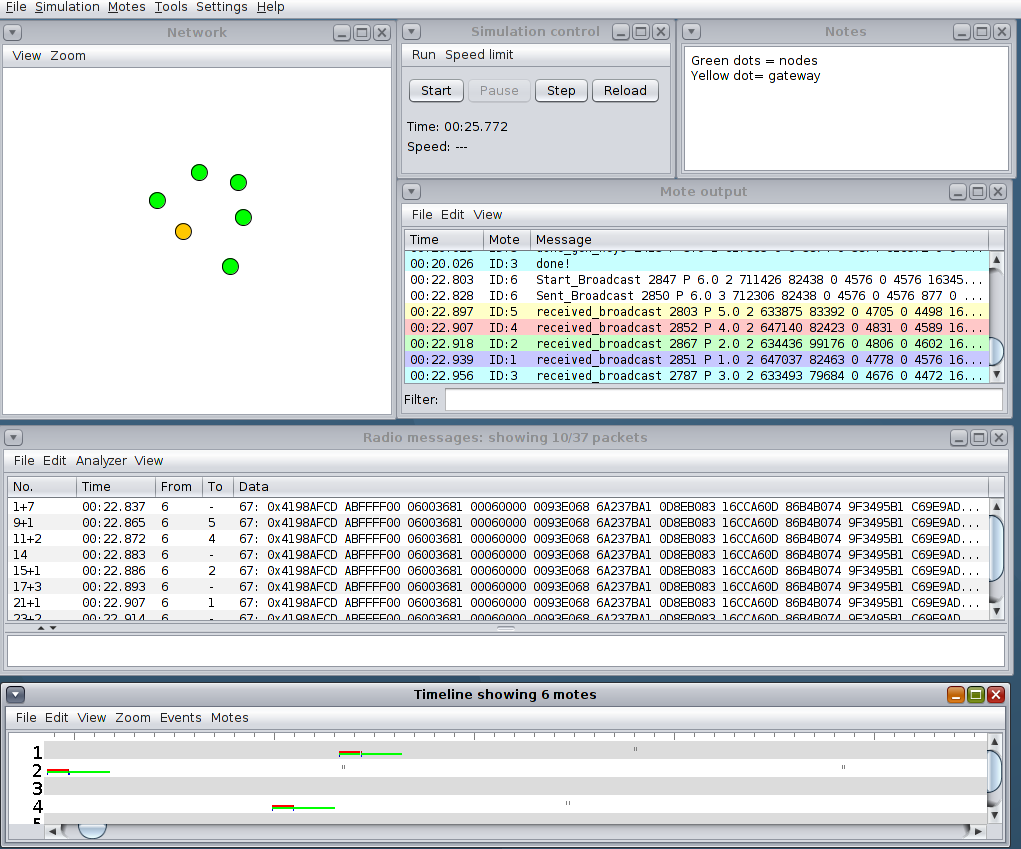
\includegraphics[width=6in]{images/cooja.png}
\caption{Cooja User Interface.}
\label{fig_cooja}
\end{figure}

The storage overhead analysis explains the memory utilized to store the parameters used by the protocol. 
The energy analysis is based on the estimate energy consumption of the computation and communication energy cost of the protocol.
Security analysis explains how the commons security threats are mitigated in the proposed solution.

\subsection{Storage Overhead}
The amount of memory required to store security parameters and key space is considered the storage cost. The total number of devices in the network is $d = m + 1$ , which is the number of nodes $m$ plus the gateway $G$. 
Calculations are performed for the \textit{secp192r1} curve ECC operations, estimating the dimension of an EC point $P = ((P_x),(P_y))$ of 48 byte.

The storage overhead slightly varies and depends on the role of the device in the network. 
In Table \ref{resourceNode} and Table \ref{resourcesGateway} are shown the parameters needed by the nodes and the gateway respectively. 
The parameters are considered using the \textit{secp192r1} elliptic curve and do not include the ones used by the authentication protocol.
Each node requires 147 bytes while the gateway has more overhead depending on the number of nodes  $n$ in the group for a total amount of $121 + 26 n$ bytes.

\begin{table}[H]
\caption{Space utilized by each parameter stored in the node using \textit{secp192r1} curve }
\label{resourceNode}
\begin{center}
\begin{tabular}{|c||c|}
\hline
 \textbf{Resource} & \textbf{Dimension (Bytes)}\\
\hline
\textit{Public Key} & 48\\
\hline
\textit{Private Key} & 24\\
\hline
\textit{Group ID} & 1\\
\hline
\textit{Shared Secret (with gateway)} & 24\\
\hline
\textit{Group Secret} & 24\\
\hline
\textit{MSK} & 24\\
\hline
\textit{Gateway's address}  & 2\\
\hline
\end{tabular}
\end{center}
\end{table}

\begin{table}[H]
\caption{Space utilized by each parameter stored in the gateway using \textit{secp192r1} curve }
\label{resourcesGateway}
\begin{center}
\begin{tabular}{|c|c|}
\hline
 \textbf{Resource} & \textbf{Dimension (Bytes)}\\
\hline
\textit{Public Key} & 48\\
\hline
\textit{Private Key} & 24\\
\hline
\textit{Group ID} & 1\\
\hline
\textit{Shared Secrets (with nodes)} & $24 \times n$\\
\hline
\textit{Group Secret}  & 24\\
\hline
\textit{MSK} & 24\\
\hline
 \textit{Nodes'  addresses} & $2 \times n$\\
\hline
\end{tabular}
\end{center}
\end{table}


\subsection{Energy Consumption Analysis}
%%%%%%%%%%%%EDIT
The performance analysis represents a major concern at this time and it is based on two key factors: the estimated energy consumption of the computation and communication energy cost of the protocols.
For the potential enormous number of IoT devices, this will help saving the energy significantly in a long term. 
For disposable-battery-powered devices, using efficient protocol means changing battery less often, which is a challenge faced by some kind of devices (i.e., devices deployed in hazardous environments or in location difficult or impossible to access frequently). 
This helps reducing battery consumption which should be recycled in certain way.
The energy consumption for each phase is calculated as follows:
%%%%%%%%%%%%%%
\begin{center}
    $energy\_consumption=\frac{Energest\_value \times current \times voltage}{RTIMER\_SECOND \times runtime}$
\end{center}

where \textit{RTIME\_SECOND} represents the number of clock ticks per second, and the values of the current and voltage are obtained from the datasheets as shown in Table \ref{tmote}.
The \textit{Energest\_Value} is the number of  MCU clock ticks (in this case: \textit{MSP430} ) required to perform common tasks like CPU usage and messages transmission or reception. 

\begin{table}[H]
\caption{Energy consumption and duration for each step of the protocol using \textit{secp192r1} curve ECC operations .}
\label{energyTime}
\begin{center}
\begin{tabular}{|c|c|c|}
\hline
& \textbf{Energy (mJ)} &  \textbf{Duration (s)}\\
\hline
\textbf{ECDH} & 19.02 & 19.220\\
\hline
\textbf{EC Point Multiplication}& 19.02 & 19.199\\
\hline
\textbf{HMAC}& $\approx0$ & 0.010\\
\hline
\textbf{AES Encrypt}& $\approx0$ & 0.010\\
\hline
\textbf{AES Dencrypt}& $\approx0$ & 0.014\\
\hline
\end{tabular}
\end{center}
\end{table}

At the node's side the complete computational overheads remain constant, irrespective of the size of the secure group.
The complete computation energy for the proposed protocol is approximately $112 mJ$ where approximately $52.8 mJ$ are spent for communication purposes. 
In Table \ref{energyTime} is shown how much time and energy are spent during each phase. 

Our protocol consumes around 6.25\% less energy than the \textit{protocol 2} in \cite{Porambage2015}.
Considering two Zinc-carbon AA batteries of 1.5 V nominal voltage and 800 mAh average capacity, the available energy is 8640 J. Consequently, this value correspond to 0.0013\% of the total available energy for one complete execution of our protocol. 
This  implies that the group key establishment phase can be executed around 77143 times.

As shown in Table \ref{energyCons}, the number of operations performed at the node side is less in the proposed protocol than the one compared with.

Compared to other protocols, the proposed one keeps the computation overhead at the node's side constant and not dependent on the number of nodes in the group.
\begin{table*}[h]
\caption{Computational overhead during each step.}
\label{energyCons}
\begin{center}
\begin{tabular}{|c|c|c|}
\hline
 & \multicolumn{2}{c|}{ \bf Node Computation Overhead}\\
\hline
\textbf{Phase} & \textbf{Proposed Protocol} & \textbf{Protocol 2 \cite{Porambage2015}}\\
\hline
 MSK establishment &  $(HMAC \approx 0) + (AES_{D}\approx0) + PM$ & $4PM + 3PA$\\ 
\hline
 Adding new node &  $(HMAC \approx 0) + (AES_{D}\approx0) + PM$ & $4PM + 3PA$\\
\hline
 Removing nodes &  $(AES_{D}\approx0) + PM$ & $4PM + 3PA$\\
\hline
\end{tabular}
\end{center}
\end{table*}

\subsection{Security Analysis}
In the security analysis are considered two type of attacker: passive and active attacker.
A passive adversary is able to only eavesdrop the ongoing communication between the nodes and the gateway trying to learn some useful information and can read all the public parameters.
As explained in Section \ref{theory:ECC}, due to the ECDL assumption is hard to compute private parameters knowing the public ones.
Therefore, learning something useful by eavesdropping the communication results infeasible since a private key is needed to derive a shared secret or the group key.

An active adversary might impose MITM (Man In The Middle) attacks during the key establishment process.
In the proposed schema, MITM attack resistance is provided by including a context-based authentication using a fuzzy commitment scheme.
An attacker, during the key establishment, needs to generate a key $\kappa$ and to use it together with his shared secret $s$ in order to perform a MITM attack. 
In fact, during the key establishment phase, the node which wants to join the group has to include a value generated with $HMAC(\kappa , s)$ , and the gateway will restore that value using his own value $\kappa$.
To generate a valid value $\kappa$ the attacker needs to get similar ambient data to the ones gotten from gateway, which means be located "close" to it.
An approach is to perform a brute force attack in order to get a valid value $\kappa$ but this means that the attacker has to try a prohibitively large number of combinations, since the commitment value is considered a random value.
It is assumed that devices located in the same ambient are considered trusted and then able to participate to the group-key establishment. 

An active attacker might try to illegitimately compute the group secret to fake the membership but, choosing a large prime $q$ for the elliptic curve, this attack is rendered impossible due to the huge amount of points on the curve to test.

In this thesis is not proposed a solution to the physical examination of the nodes from an attacker.
Moreover, the proposed scheme do not provide a solution to denial of service attacks.



	%\input{text/discussion.tex}
	% $Id: discussion.tex 142 2012-12-22 10:41:32Z danbos $
\chapter{Conclusions}
\label{ch:conclusion}
This thesis presented the design of a lightweight group-key establishment protocol with context-based authentication.
First the feasibility to utilise contextual information to authenticate devices in the same environment in order to remove the necessity of any interaction with human or pre-sharing keys to establish a secure channel has been studied.
The approach has been exemplified for ambient audio and other context sources, using data collected by a set of seven devices assembled with the sensors in two different environments.
To generate a unique authentication secret key among the devices in the same environment a fuzzy commitment scheme has been used and adapted in its noise tolerance through its error correcting code parameters.
The scheme has been tested using two different kind of fingerprints: one generated from the audio and one generated from the other sensors.
The results show that it is difficult to neglect authentication when the sensing is performed in different times.
This is due to the absence of events which generate high entropy on the sensed ambient features.
However, when devices are located in different environments, it results easily feasible to not authenticate them due to the highly different generated fingerprints.
This answers to the research question RQ2, underlying the difficulties encountered for the context-based authentication design in environments with absence of high entropy events.

This thesis also presented the proof-of-concept implementation of the protocol for Contiki and constrained devices, followed by an evaluation of its performances.
The scheme leverages the notion of one-way cryptographic accumulators to enable end nodes connected to a common gateway to establish and manage a secure group channel which guarantees forward and backward secrecy.

The proposed protocol has been tested using Cooja and Tmote Sky with an actual multicast group.
Tmote Sky, as the constrained devices used in this thesis, is a well-known device which is supported by Cooja. 
Tmote Sky has limited support for cryptographic operations and, in order to implement the protocol, all cryptographic operations needs to be implemented in application level. 
As consequence, the memory occupancy and the computing time is higher on the node and gateway side.
The protocol's performance in term of total energy spent by the nodes has been evaluated and compared to similar solutions.
The results show an increment of performances in terms of computation overhead and energy consumption, proving the efficiency of the proposed solution for group-key management on resource constrained devices.
This provide an answer to the RQ1, showing that the proposed protocols could improve performances and being implemented on resource-constrained devices.

\section{Ethical and social considerations}

IoT  applications  are  becoming  part  and  parcel  of  our  daily  lives  in  various  areas such as healthcare, industrial automation and transports. 
The number of IoT devices is growing day by day, sharing between them an enormous amount of users' personal information.
Protecting them using appropriate authentication and key management protocols becomes necessary to guarantee security services such as safety, confidentiality and privacy, and the protocols presented in this thesis work could be integrate in security suites.
In order to be trusted by the users it is important that the IoT applications presents strong built-in security mechanisms and this motivates the high applicability of the presented solutions.
Moreover, improving the efficiency in terms of power consumption of these protocols brings benefits in terms of costs and less waste of batteries.

An ethical aspect to consider is the design of protocols which can include weaknesses which can be exploited in a second time by third parties \cite{DorothyE.DenningandMilesSmid1994KeyMagazine} or to use them for malicious activities also known as kleptographic purposes \cite{Young2010MaliciousAspects}.

The protocols presented here are based on public cryptographic primitives and the security services they claim to provide are duly proved. 
Moreover, a justification of why and how they are useful to secure IoT applications is thoroughly
provided. 


%Judgement based on subject based aspects (aka your work..)
%Judgement based on Social aspects
%Judgement based on Ethical aspects






\section{Future work}
The thesis work analyzes the feasibility of authentication solutions based on context information observed by IoT devices and proposes a group-key management protocol based on this approach. 
The data for the analysis has been obtained from two environments and using the same deployment settings for each device.
This framework needs to be based on the  analysis  of  large-scale empirical measurements in a wider range of typical deployment settings of IoT devices  in  different environments. 

The authentication keys generated from the sensors data and from the audio have been considered separately. 
Therefore, a future step is to generate an unique and improved fingerprint form the different data.

The key management solution proposed in this work is based on classical cryptographic primitives which rely on problems hard to solve by non-quantum computers.
Building a quantum-safe solution is a potential future work, before quantum computers will be a reality able to break the used cryptographic primitives.

The implementations effectuated during the thesis work, as explained in \ref{sec:scope} are considered Proof of Concept. 
One might also consider applying a different third-party library and compare different levels of security.
















    \printbibliography
    \clearpage
    \listoffigures
    \clearpage
    \listoftables
    %\clearpage
    %\lstlistoflistings
\iffalse
	\appendix

    \chapter{Included Publications}
    This appendix chapter contains the following publication of the author in full-text form in the outlined order:

    \begin{enumerate}[label=\Roman*]
        \item Nico Ferrari, Teklay Gebremichael, Ulf Jennehag, and Mikael Gidlund{\"o}m. "Lightweight Group-Key Establishment Protocol for IoT Devices: Implementation and Performance Analyses". In: \textit{2018 Fifth International Conference on Internet of Things: Systems, Management and Security, IEEE, 2018}
    \end{enumerate}
	
	
	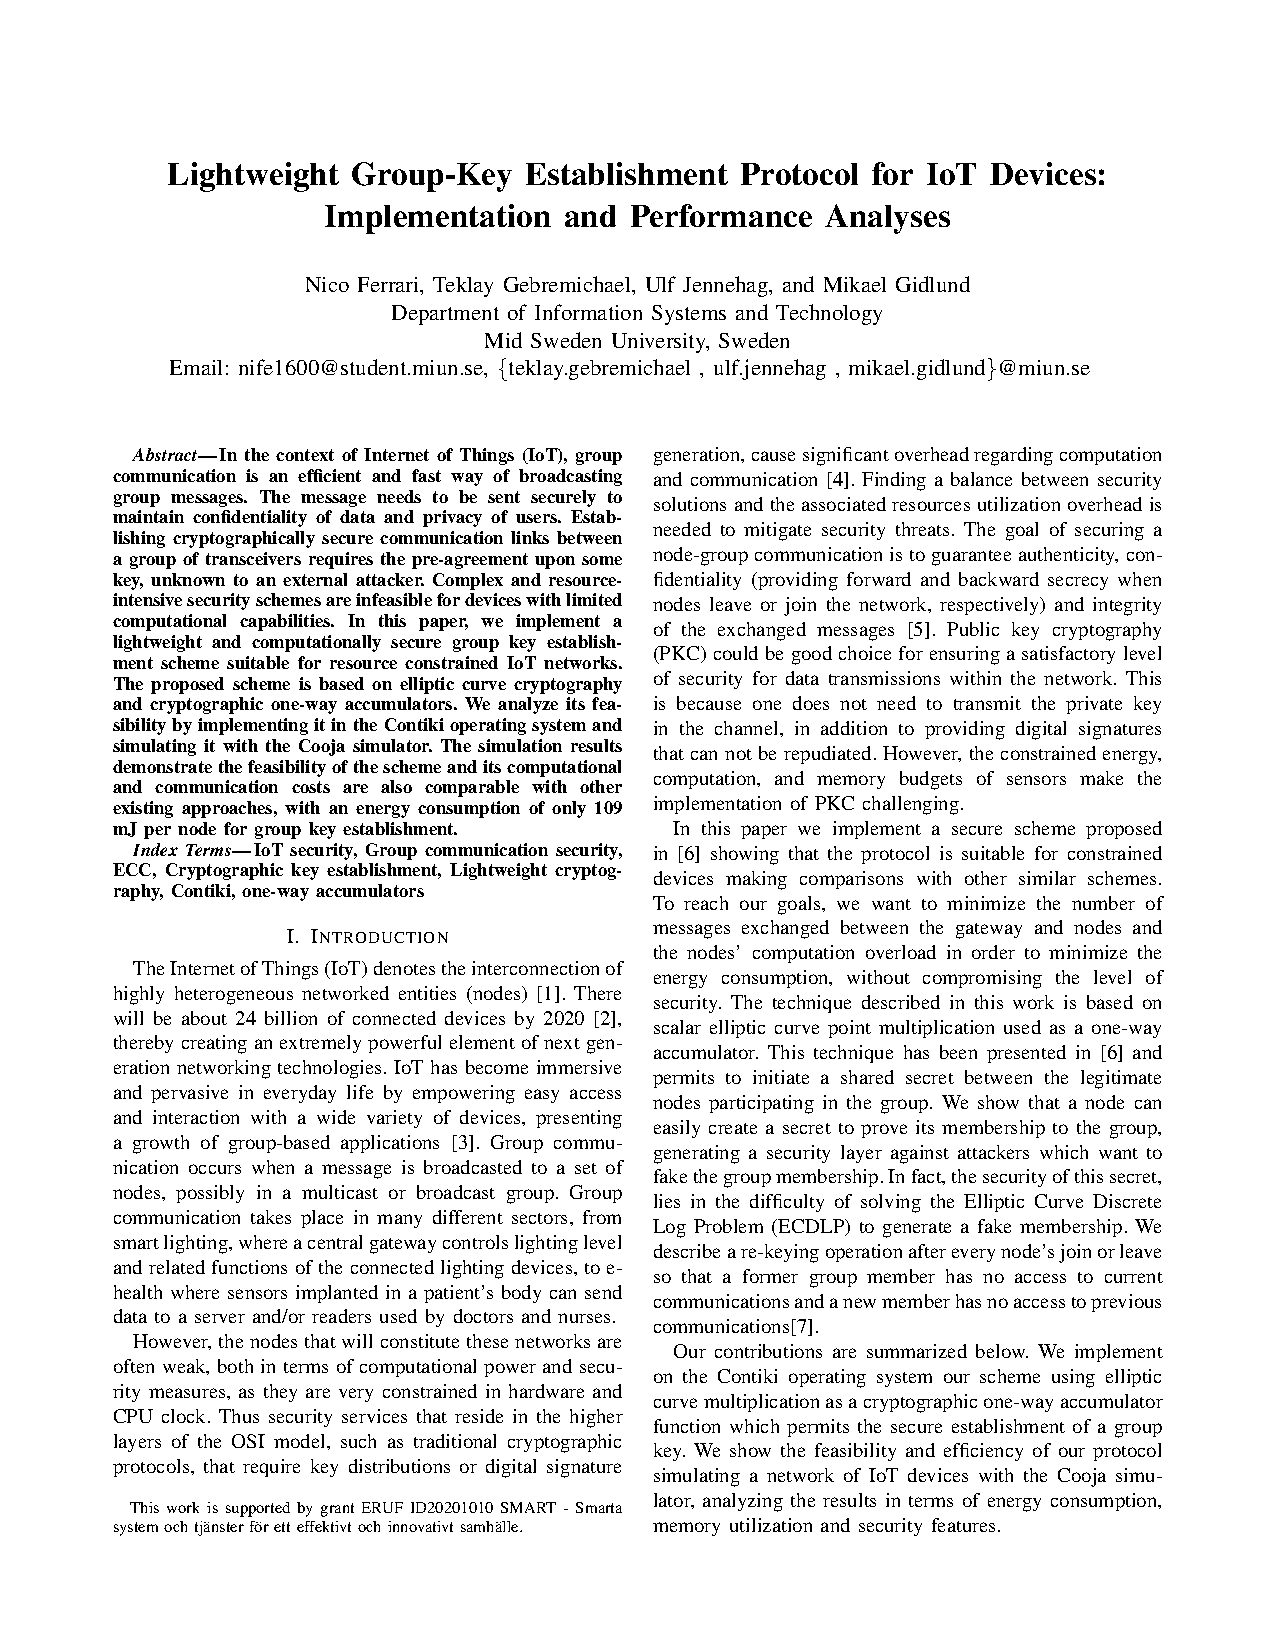
\includepdf[pages=-]{docs/Group_Exchange_Key_Protocol.pdf}
\fi

	

	\backmatter
	% index etc.
\end{document}